\documentclass[11pt]{article}
\usepackage{latexsym}
\usepackage{amsmath}
\usepackage{amssymb}
\usepackage{amsthm}
\usepackage{epsfig}
\usepackage{bm}
\usepackage{scrextend}
\usepackage[tight]{subfigure}

\usepackage{amsmath}
% \usepackage{algorithmicx}
\usepackage{algorithm}
\usepackage{algpseudocode}

\DeclareMathOperator*{\minimize}{min}
\DeclareMathOperator*{\maximize}{max}
\DeclareMathOperator{\sign}{sign}


 %on linux you may need to run sudo apt-get install texlive-full to install algorithm.sys

\usepackage{verbatim}

\newcommand{\handout}[5]{
  \noindent
  \begin{center}
  \framebox{
    \vbox{
      \hbox to 5.78in { {#1} \hfill #2 }
      \vspace{4mm}
      \hbox to 5.78in { {\Large \hfill #5  \hfill} }
      \vspace{2mm}
      \hbox to 5.78in { {\em #3 \hfill #4} }
    }
  }
  \end{center}
  \vspace*{4mm}
}

\newcommand{\lecture}[5]{\handout{#1}{#2}{#3}{#4}{#5}}
\newcommand{\collision}[0]{\mathrm{collision}}
\newcommand{\nocollision}[0]{\overline{\collision}}
\newcommand{\argmax}[1]{\underset{#1}{\operatorname{arg}\,\operatorname{max}}\;}
\newcommand{\argmin}[1]{\underset{#1}{\operatorname{arg}\,\operatorname{min}}\;}

\newcommand*{\QED}{\hfill\ensuremath{\square}}

\newtheorem{theorem}{Theorem}
\newtheorem{corollary}[theorem]{Corollary}
\newtheorem{lemma}[theorem]{Lemma}
\newtheorem{observation}[theorem]{Observation}
\newtheorem{proposition}[theorem]{Proposition}
\newtheorem{definition}[theorem]{Definition}
\newtheorem{claim}[theorem]{Claim}
\newtheorem{fact}[theorem]{Fact}
\newtheorem{assumption}[theorem]{Assumption}
\newtheorem{note}[theorem]{Note}


% 1-inch margins, from fullpage.sty by H.Partl, Version 2, Dec. 15, 1988.
\topmargin 0pt
\advance \topmargin by -\headheight
\advance \topmargin by -\headsep
\textheight 8.9in
\oddsidemargin 0pt
\evensidemargin \oddsidemargin
\marginparwidth 0.5in
\textwidth 6.5in

\parindent 0in
\parskip 1.5ex
%\renewcommand{\baselinestretch}{1.25}

\begin{document}

\lecture{Statistical Techniques in Robotics (16-831, S21)}{Lecture \#06
  (Wednesday, February 17)}{Lecturer: Kris Kitani}{Scribes: Haowen Shi, Fan Jia}{Online Convex Optimization (Convexity, FTL)}

\section{Review}
%This section serves as a review of the previous lecture and any other context required to frame the content of the current lecture. 

%You may format the scribes in any way you like, aside from changing font style, size and page format. Please use subsections and paragraphs to increase the readability of your notes.

%Length requirement 1-2 pages.

\subsection{Overview}

In the past lectures we have studied a few online learning algorithms including PWEA and Online Linear Classification. In this lecture we study a generalized framework of these online learning algorithms called \textit{Online Convex Optimization} (OCO). We explain why OCO is a generalization of online learning in section \ref{sec:rel_online_learning}.
% \begin{figure}[h]
%     \centering
%     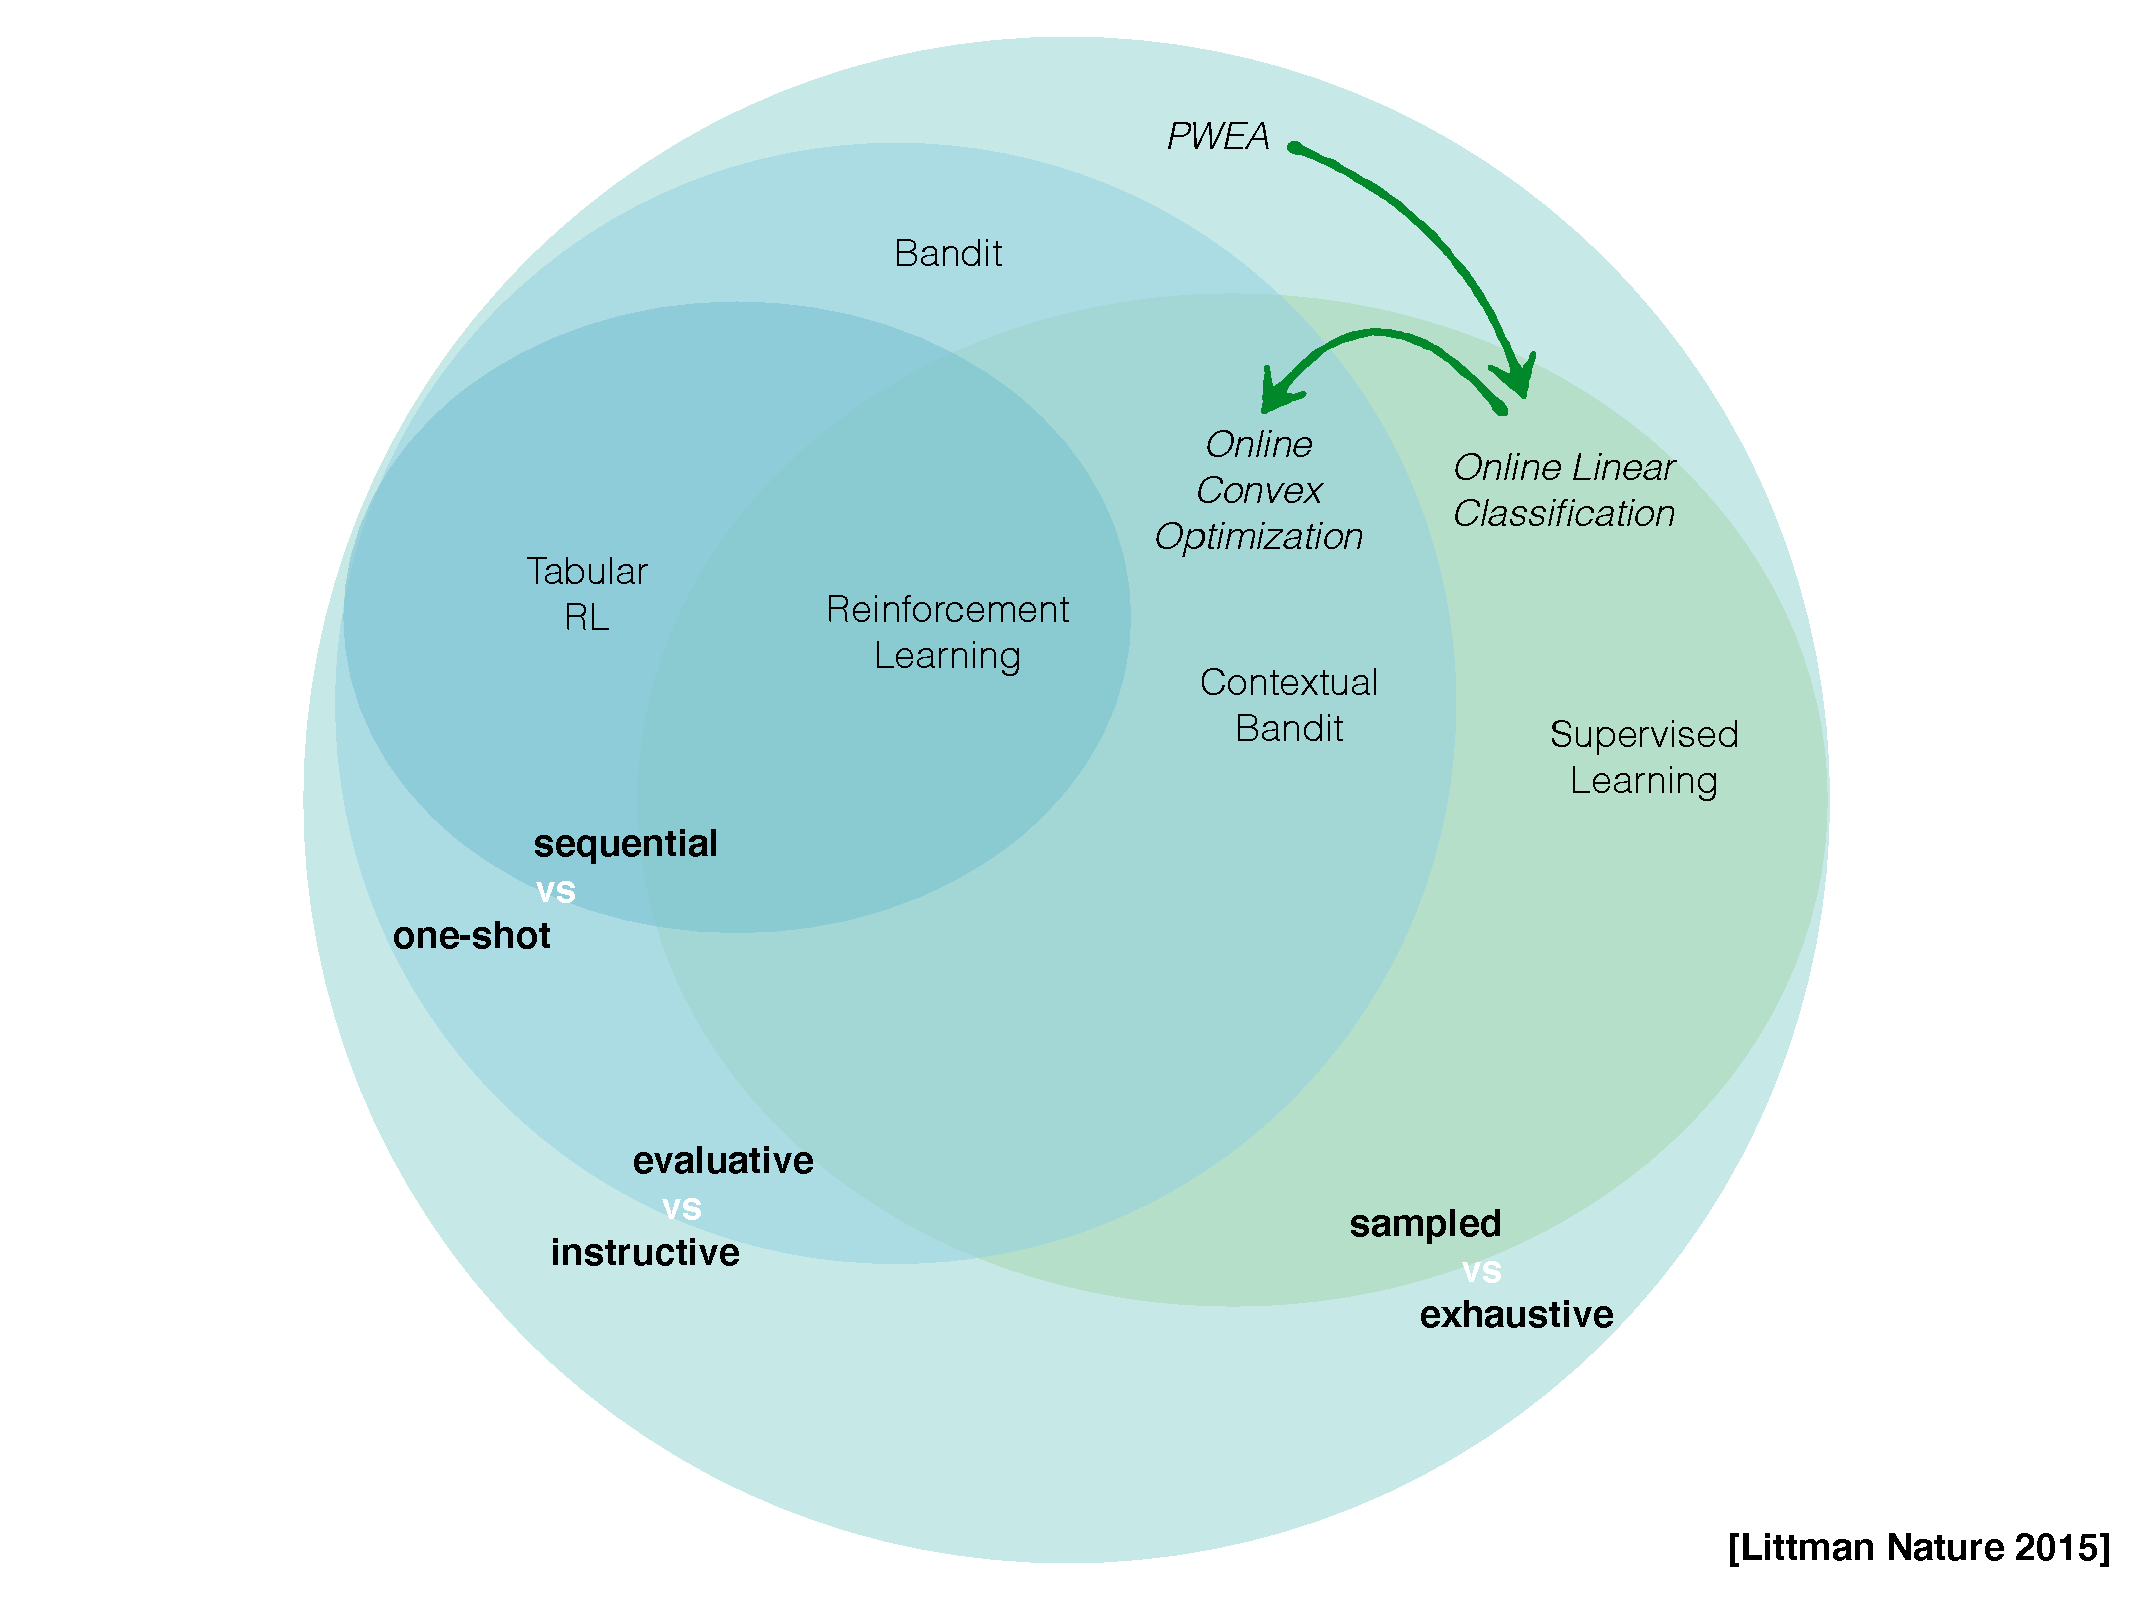
\includegraphics[width=0.6\textwidth]{figure/where_we_are.pdf}
%     \caption{Where we are in the class}
%     \label{fig:where_we_are}
% \end{figure}

\begin{figure}[h]
\centering
\begin{minipage}[t]{.5\textwidth}
    \centering
    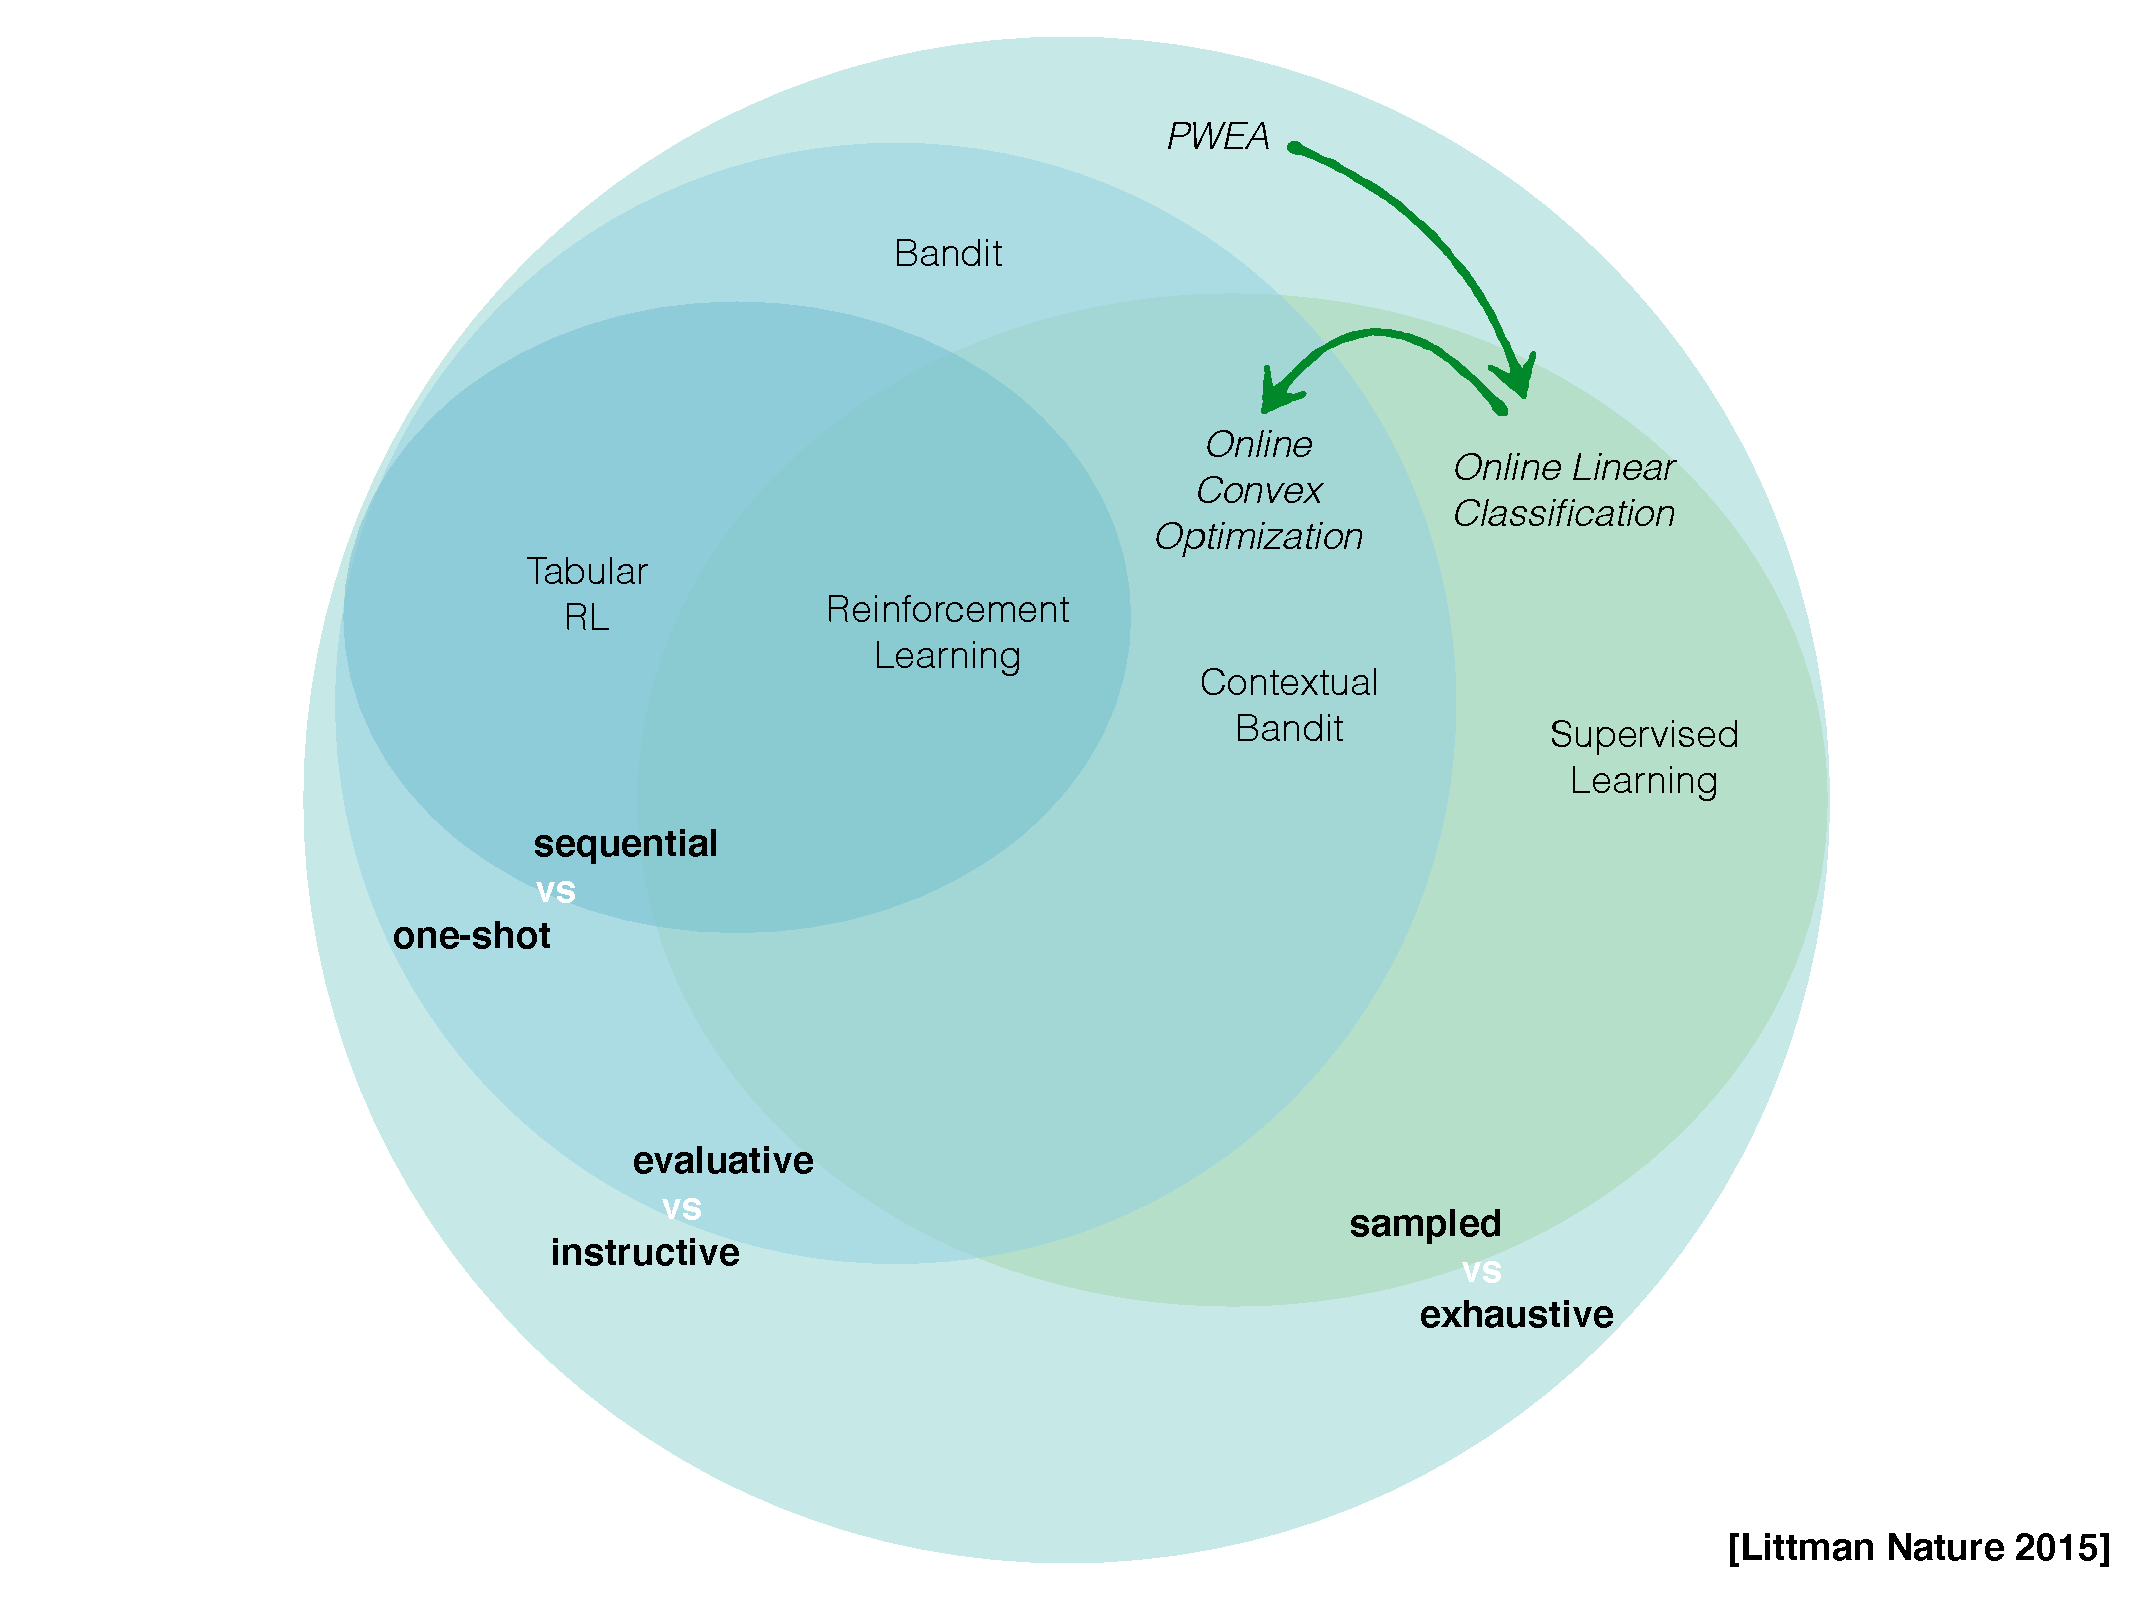
\includegraphics[width=.99\linewidth]{figure/where_we_are.pdf}
    \caption{Where we are in the class}
    \label{fig:where_we_are}
\end{minipage}%
\begin{minipage}[t]{.5\textwidth}
    \centering
    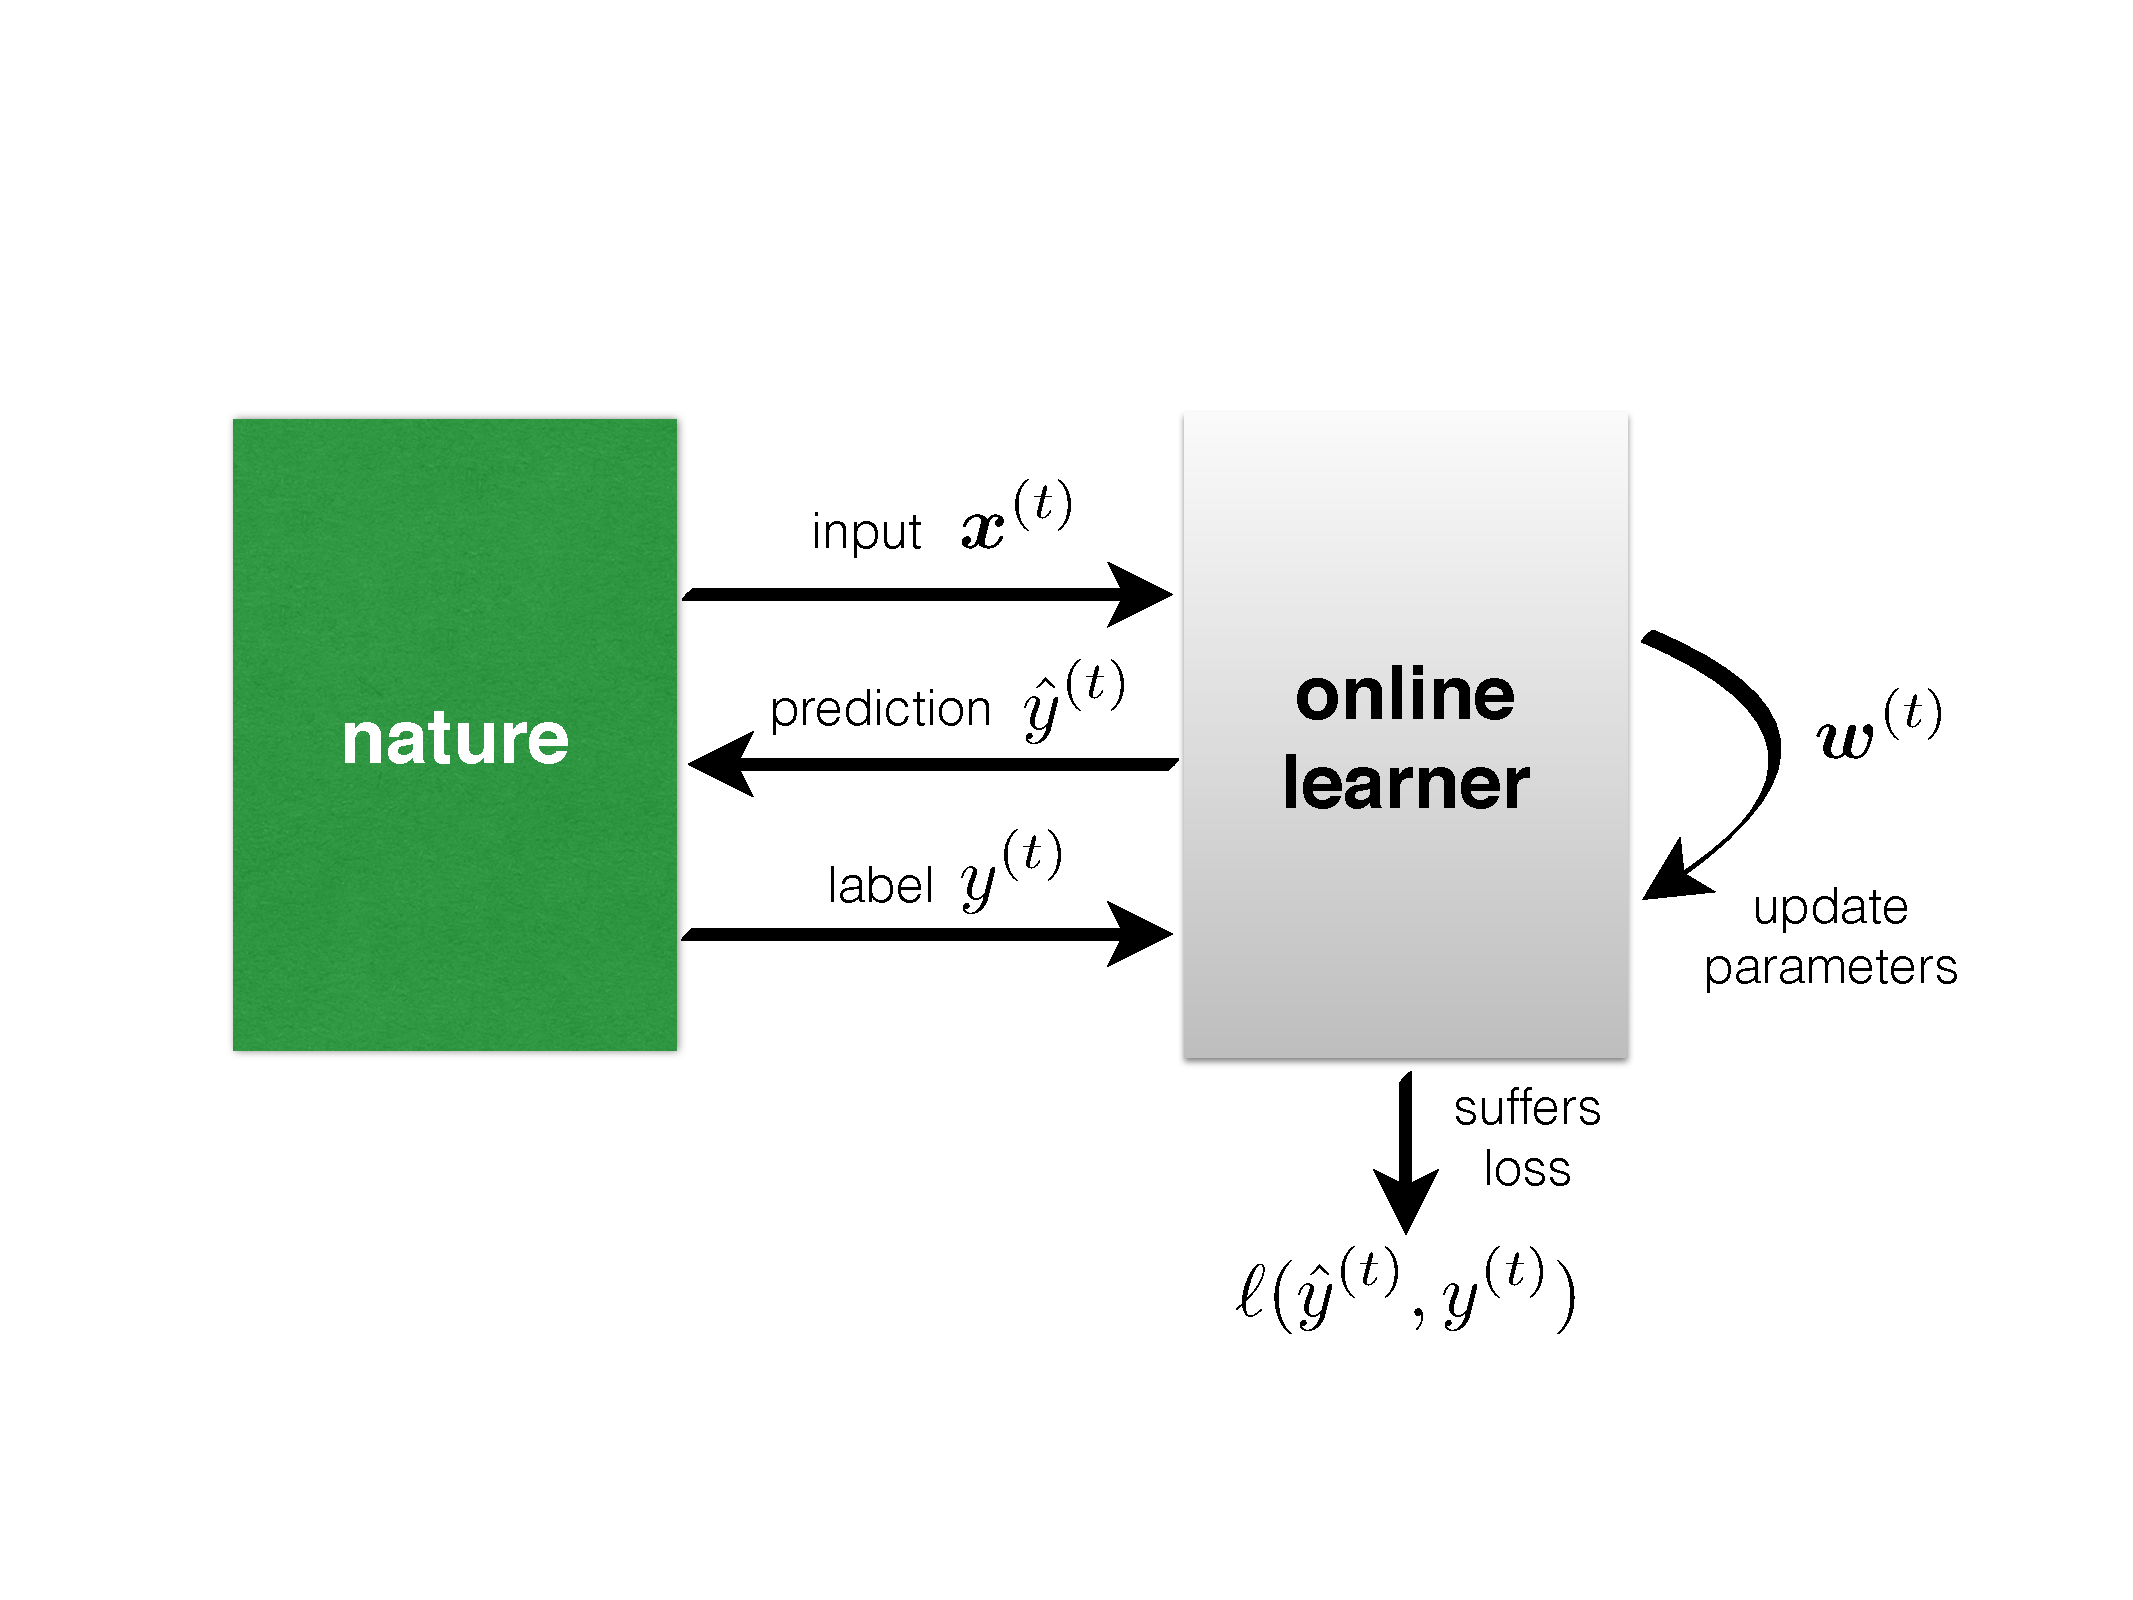
\includegraphics[width=.90\linewidth]{figure/online_learning.pdf}
    \caption{Online learning framework}
    \label{fig:online_learning}
\end{minipage}
\end{figure}

\subsection{Online Learning}
In online learning, the prediction model is incrementally improved over multiple iterations. The events that happen in each iteration is illustrated in Fig. \ref{fig:online_learning}. At each time step $t$, the learner receives input $\bm{x}^{(t)}$, makes a prediction $\hat{y}^{(t)}$ and then receives the true outcome $y^{(t)}$ from the environment. The loss function $l(\hat{y}^{(t)}, y^{(t)})$ is evaluated by the learner to produce a loss which drives the update of model weights $\bm{w}^{(t)}$.

% \begin{figure}[h]
%     \centering
%     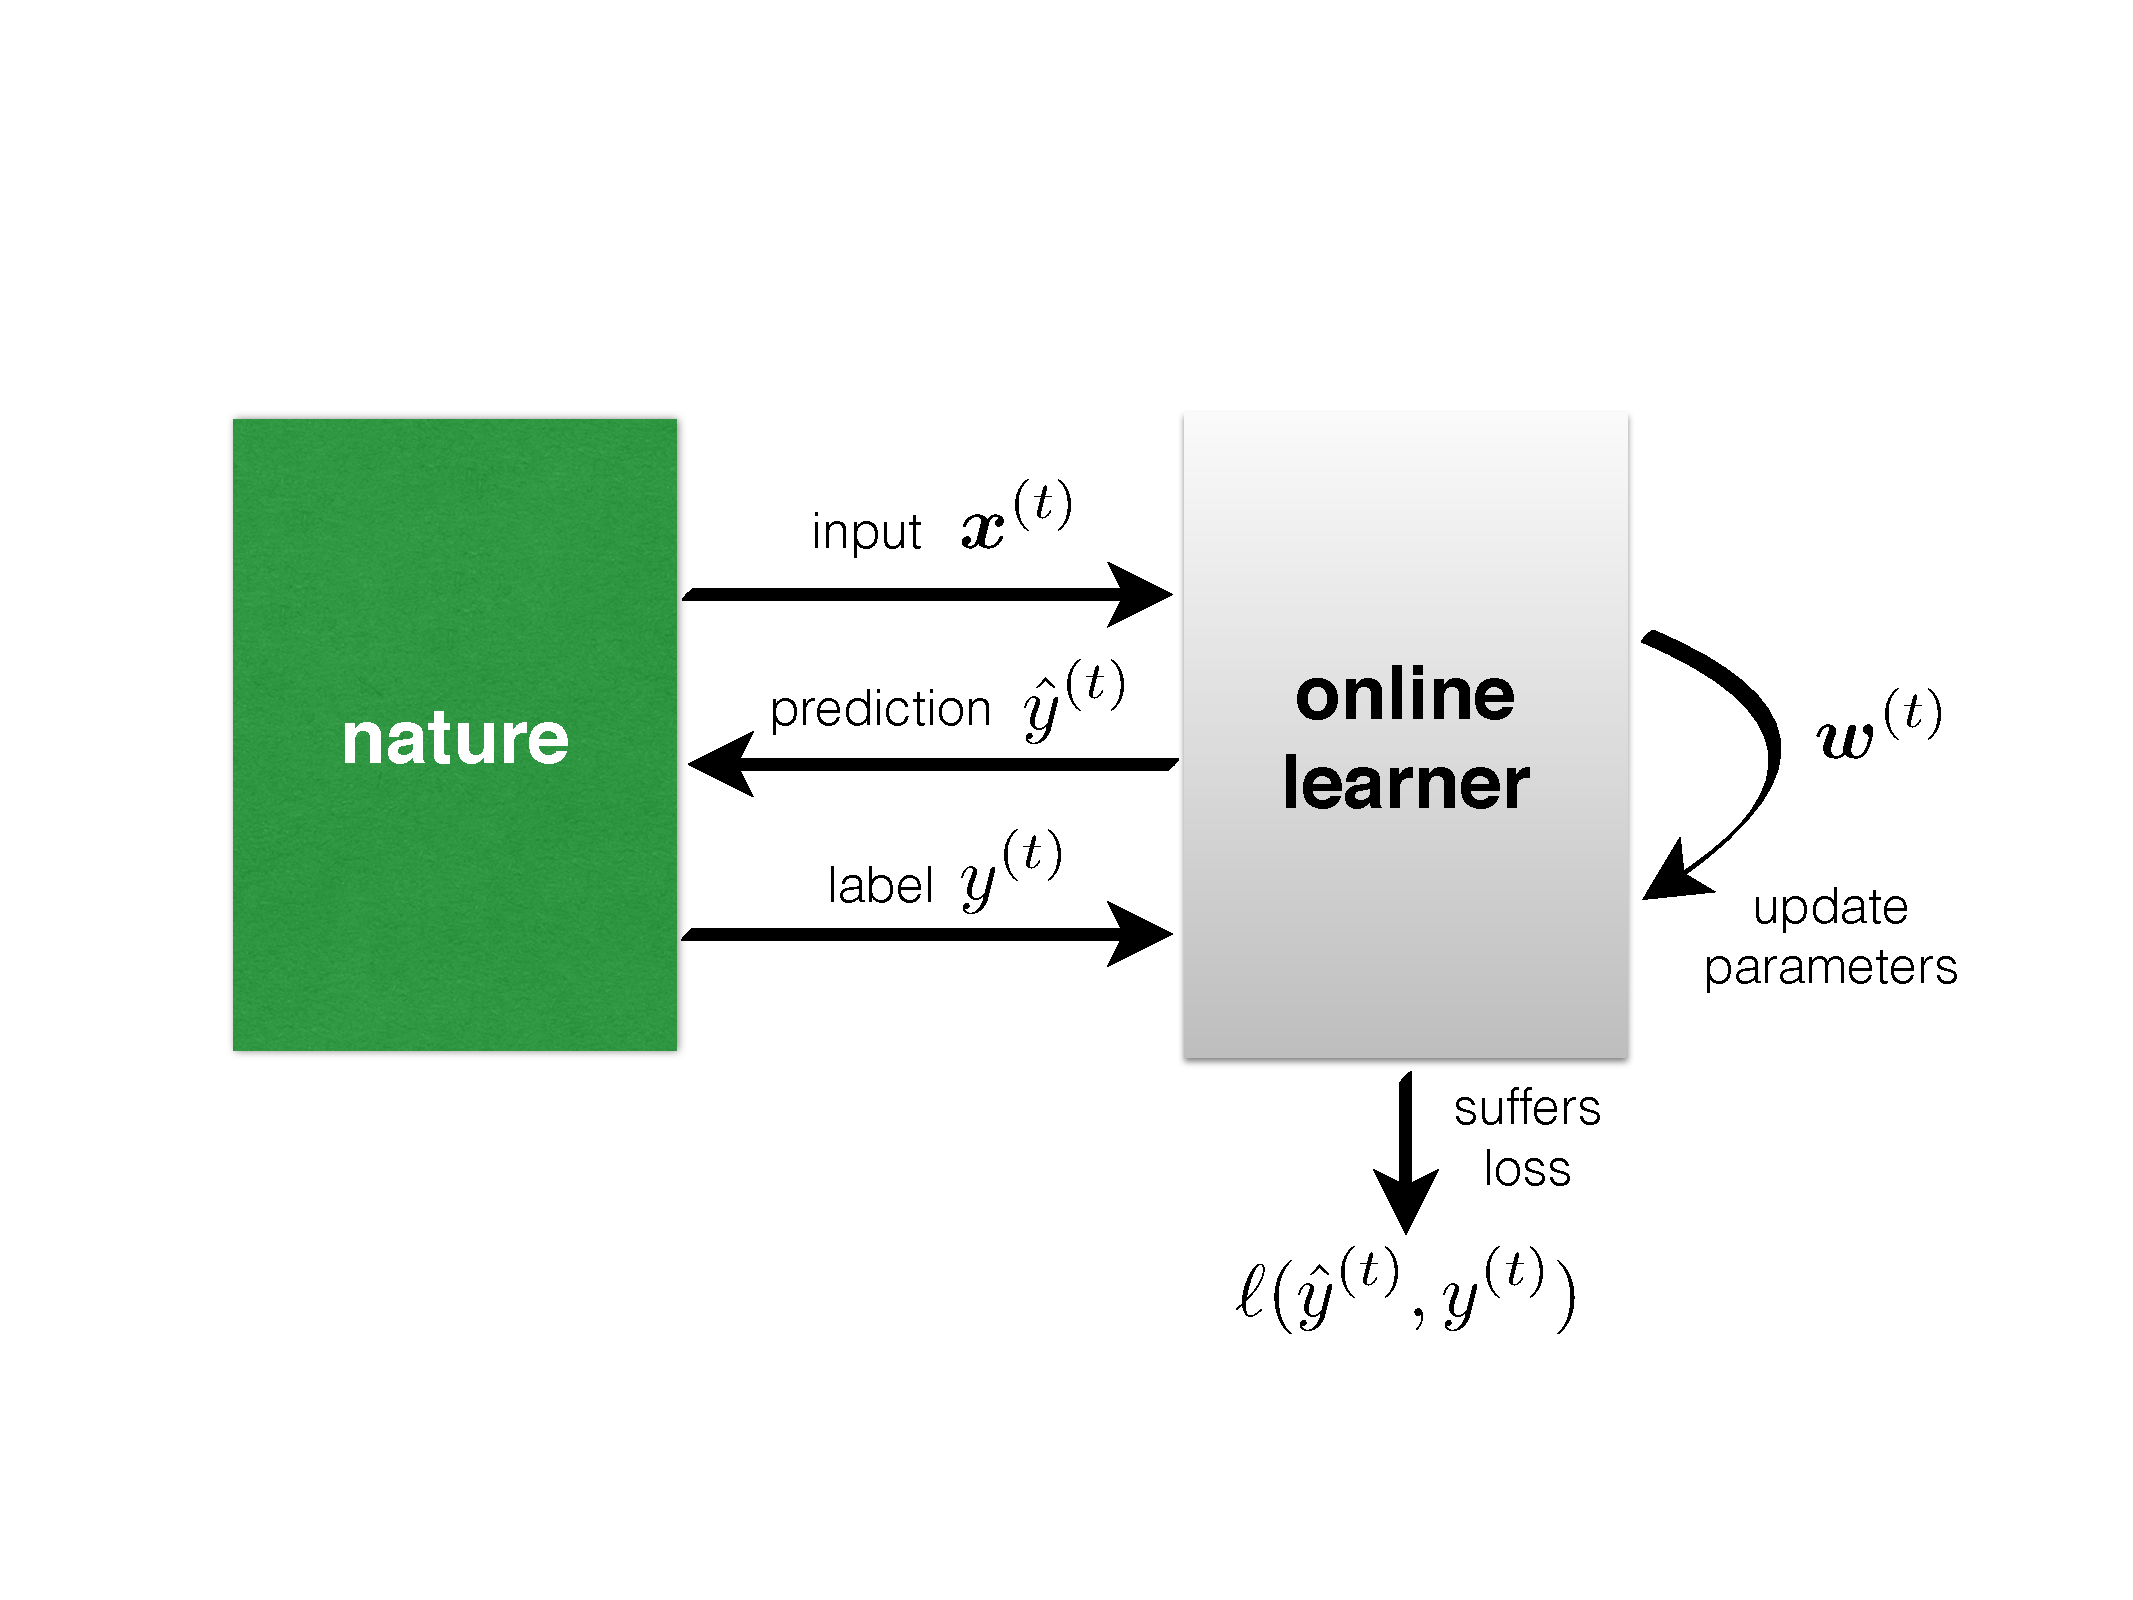
\includegraphics[width=0.6\textwidth]{figure/online_learning.pdf}
%     \caption{Online learning framework}
%     \label{fig:online_learning}
% \end{figure}

In previous lectures we have learned about two main classes of online learning:
\begin{itemize}
    \item Prediction with Expert Advice (PWEA)
    \begin{itemize}
        \item Greedy / Consistent Algorithm
        \item Halving Algorithm
        \item Weighted Majority Algorithm
        \item Randomized Weighed Majority Algorithm
    \end{itemize}
    \item Online Linear Classification
    \begin{itemize}
        \item Perception Algorithm
        \item Winnow Algorithm
    \end{itemize}
\end{itemize}

\begin{algorithm}[H]
\caption{Perceptron algorithm}
\label{algo:perceptron}
\begin{algorithmic}[1]
\State $\bm{w}^{(1)} \leftarrow \mathbf{0}$ \hfill $\triangleright$ Weight initialization
\For{$t=1,\;\cdots,\;T$}
\State \textsc{Receive} ($\bm{x}^{(t)}\in \mathbb{R}^N$) \hfill $\triangleright$ Receive expert predictions
\State $\hat{y}^{(t)} = \text{sign}\Big(\langle \bm{w}^{(t)}, \bm{x}^{(t)} \rangle\Big)$ \hfill $\triangleright$ Make learner prediction
\State \textsc{Receive} ($y^{(t)}\in\{-1, 1\}$) \hfill $\triangleright$ Receive actual answer
\State $\bm{w}^{(t+1)}\leftarrow \bm{w}^{(t)} + y^{(t)} \cdot x^{(t)} \cdot\textbf{1}[y^{(t)}\neq \hat{y}^{(t)}] $ \hfill $\triangleright$ Weight update
\EndFor
\end{algorithmic}
\end{algorithm}

\begin{algorithm}[H]
\caption{Winnow algorithm}
\label{algo:winnow}
\begin{algorithmic}[1]
\State $\bm{w}^{(1)} = \{1, \ldots, 1\}$ \hfill $\triangleright$ Weight initialization
\For{$t=1,\;\cdots,\;T$}
\State \textsc{Receive} ($\bm{x}^{(t)}\in \{0,1\}^N$) 
\State $\hat{y}^{(t)} = \mathbf{1}[\langle \bm{w}^{(t)}, \bm{x}^{(t)} \rangle > N]$ \hfill $\triangleright$ Make prediction
\State \textsc{Receive} ($y^{(t)}\in\{0, 1\}$) 
\State $w_i^{(t+1)}= w_i^{(t)}(1+\beta) ^ {(y^{(t)} - \hat{y}^{(t)})\cdot x_i^{(t)}} $\hfill $\triangleright$ Weight update
\EndFor
\end{algorithmic}
\end{algorithm}

\section{Online Convex Optimization}

\subsection{The Optimization Problem}
An optimization problem is the process of finding the best solution among all feasible solutions. Given a function of variables $f(\bm{x})$, we want to find the set of variables $\bm{x}$ such that the function produces the optimal (minimum) value $\hat{\bm{x}}$.
\begin{equation*}
    \hat{\bm{x}} = \argmin{\bm{x}} f(\bm{x})
\end{equation*}
In real life, most optimization problems are also \textit{constrained} to meet a set of requirements, these constraints can fall in the following categories:
\begin{align*}
    \text{Inequality Constraint:\quad} & g(\bm{x}) \leq 0 \\
    \text{Equality Constraint:\quad} & h(\bm{x}) = 0 \\
    \text{Domain Constraint:\quad} & \bm{x} \in \mathbb{S}
\end{align*}
To solve the optimization problem, there are three high level approaches:
\begin{enumerate}
    \item Analytic solution\\[1ex]
          In some optimization problems we have a well defined objective function $f$ so we can find its minima by evaluating its gradient $\nabla f$ and setting it to zero. Analytic solution is fast and global for convex objective functions but it is not always possible because the objective function might be too complex to evaluate or sometimes hidden to us.
    \item Brute force search\\[1ex]
          Brute force search works well in small domain sizes and always obtains globally optimal solutions. The computation soon becomes intractable as the domain size grows so it's not always feasible.
    \item Numerical methods\\[1ex]
          Solving optimization problems using numerical methods is very popular in the learning community because the computation cost scales well as problem difficulty grows. However, the trade off is numerical solutions are not always globally optimal because they can converge to local minima depending on the initialization.
\end{enumerate}

\subsection{Relationship with Online Learning}
\label{sec:rel_online_learning}
Online Convex Optimization is a more generalized framework for online learning. In OCO, the learner does not make any observations of the environment, it just sends a set of parameters $\bm{w}^{(t)}$ to the environment and gets a loss function $l^{(t)}$ back, as shown in Fig. \ref{fig:oco_1} and Algorithm \ref{alg:oco}. The reason we say OCO is a higher level framework is that we can easily use OCO to solve online learning problems by replacing the "nature" in Fig. \ref{fig:oco_1} with a online learning model. As illustrated in Fig. \ref{fig:oco_2}, the online learner in red is calling the online convex optimizer in gray for the prediction step to update its weights.

\begin{figure}[h]
\centering
\begin{minipage}{.5\textwidth}
    \centering
    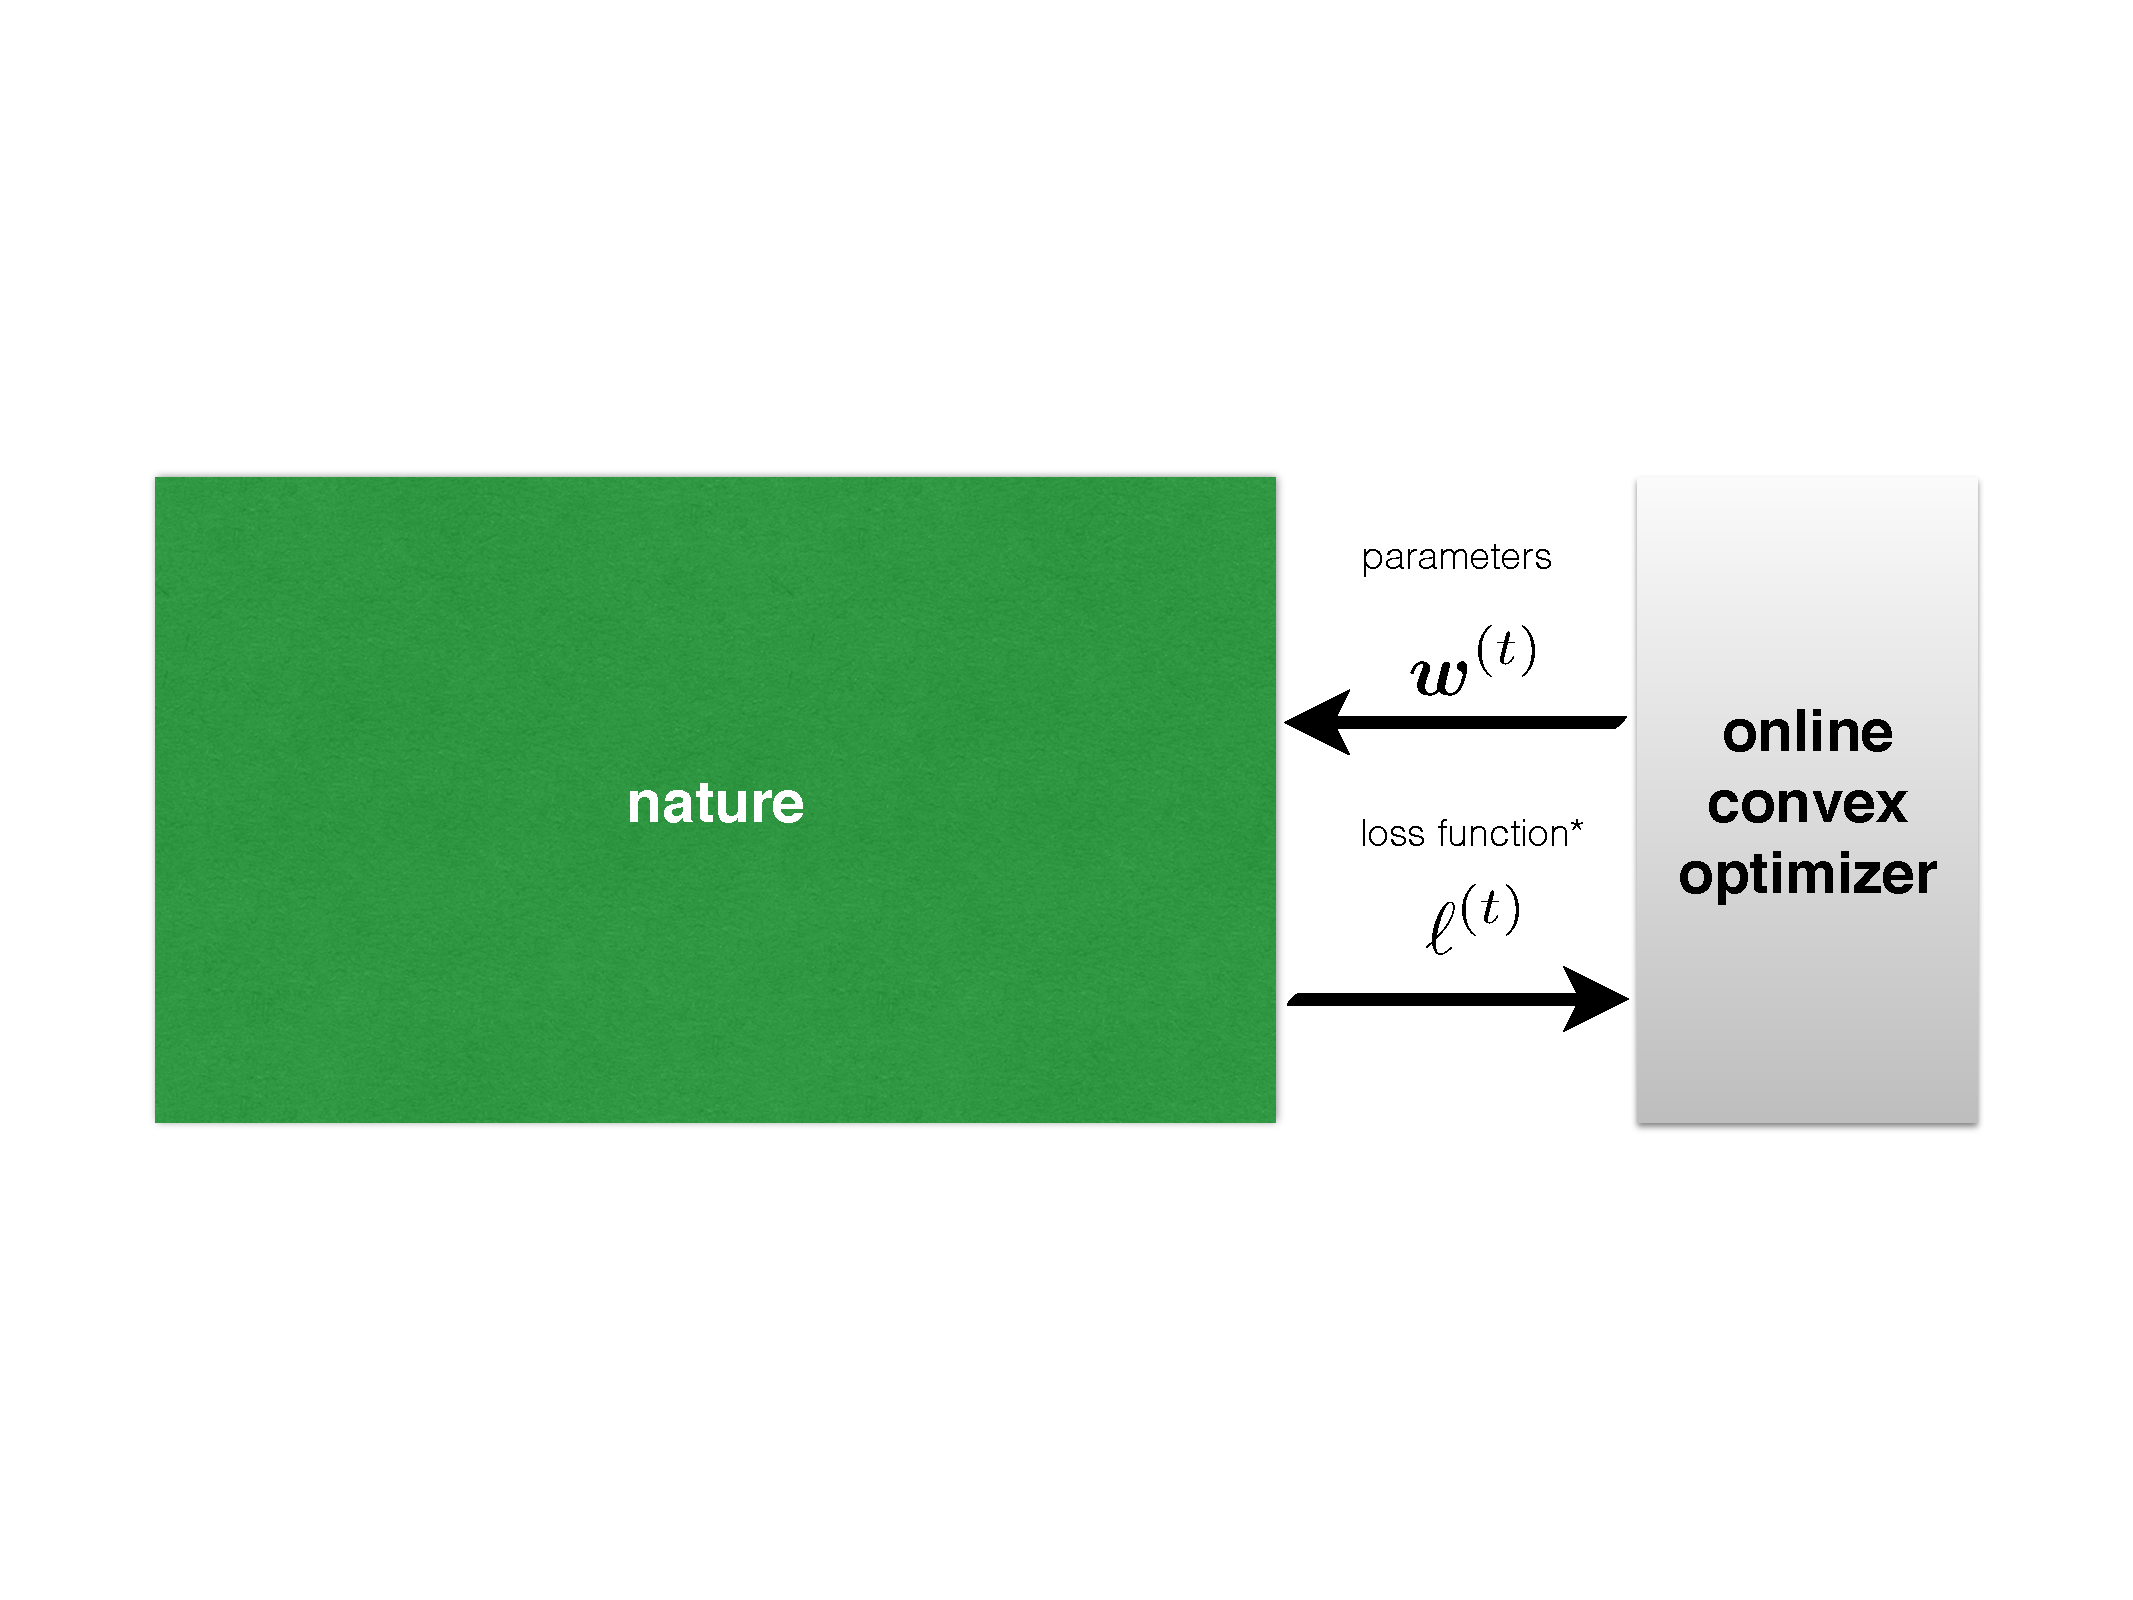
\includegraphics[width=.90\linewidth]{figure/oco_1.pdf}
    \caption{OCO framework}
    \label{fig:oco_1}
\end{minipage}%
\begin{minipage}{.5\textwidth}
    \centering
    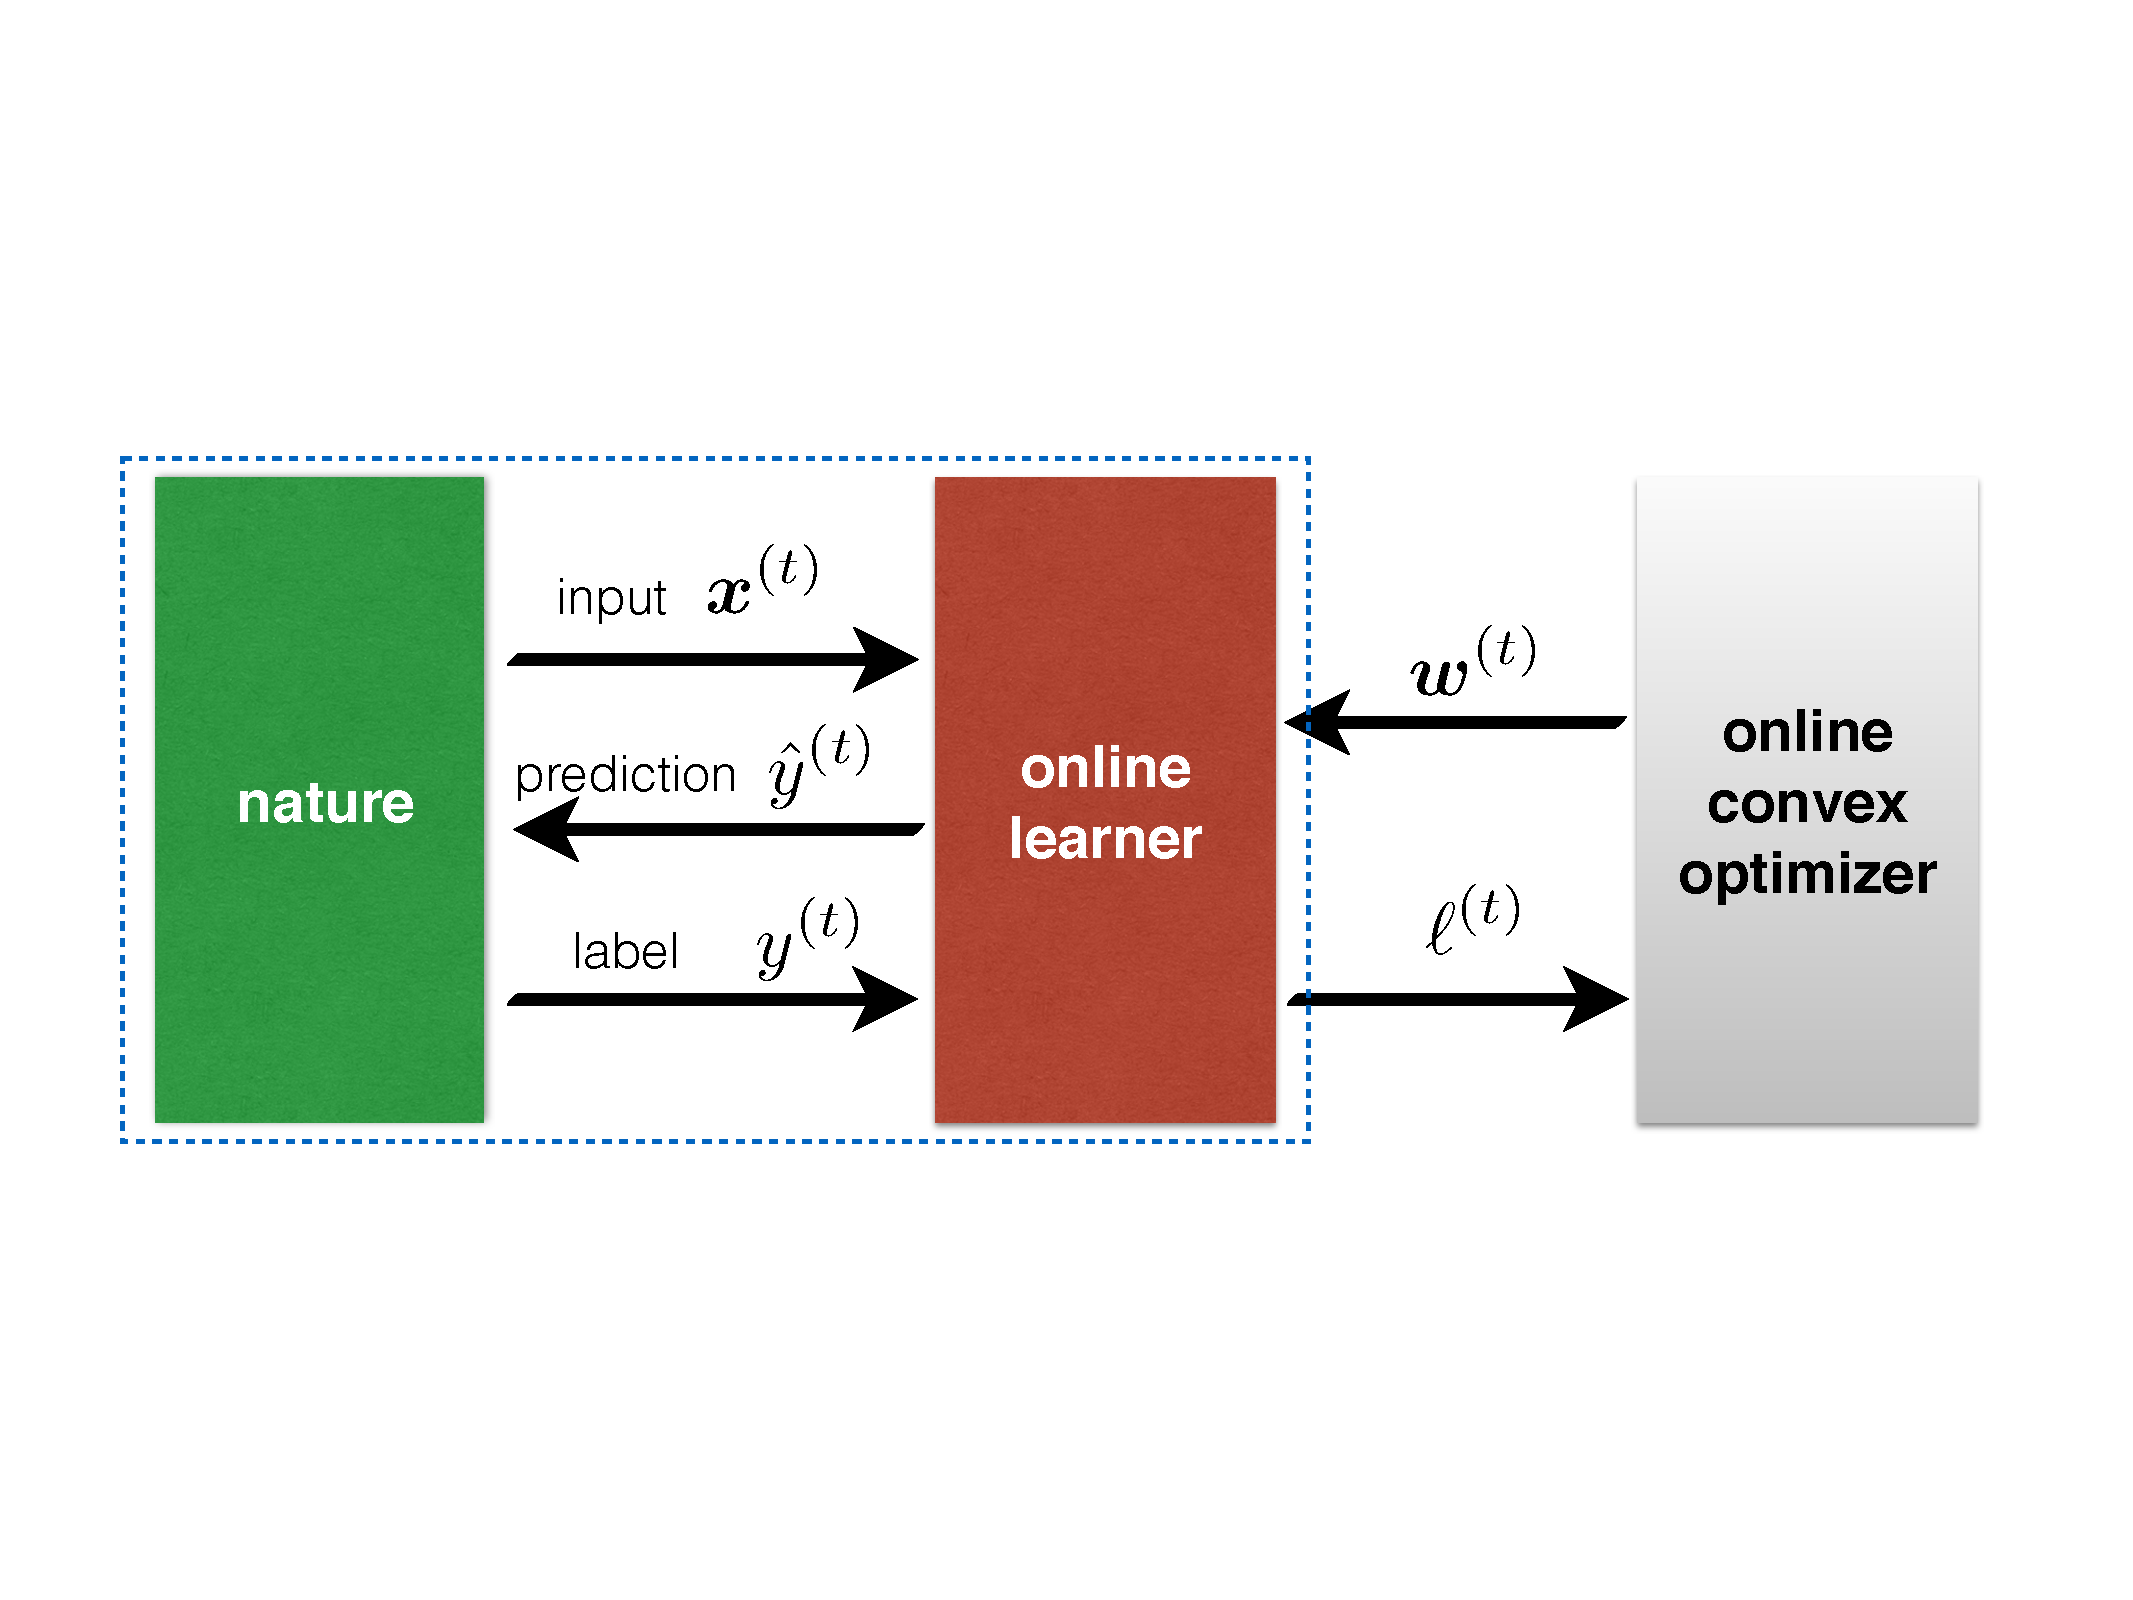
\includegraphics[width=.90\linewidth]{figure/oco_2.pdf}
    \caption{OCO is a generalization}
    \label{fig:oco_2}
\end{minipage}
\end{figure}

\begin{algorithm}
  \caption{Online Convex Optimization}\label{alg:oco}
  \begin{algorithmic}[1]
    \Function{OnlineConvOpt}{Convex set $\mathcal{S}$}
        \For{$t=1, 2,\,\cdots,\;T$}
            \State \textsc{Predict} ($\bm{w}^{(t)} \in \mathcal{S}$) \Comment{Solution space must be a convex set}
            \State \textsc{Receive} ($f_t : \mathcal{S} \rightarrow \mathbb{R}$) \Comment{Loss function must be convex}
            \State \textsc{Compute Loss} ($f_t (\bm{w}^{(t)})$)
        \EndFor
    \EndFunction
  \end{algorithmic}
\end{algorithm}

\subsection{Convex Optimization}

Generally if a optimization problem is convex, there will be a global optima which can be found faster than non-convex problems.
%This section describes when a problem is convex and how to approximate non-convex problems as convex ones.

\subsubsection{Convex Set}
A set $\mathcal{S}$ is convex if for all $\bm{w}, \bm{v} \in \mathcal{S}$, and for all $\alpha \in [0, 1]$, the following holds:
\begin{equation*}
    \alpha \bm{w} + (1 - \alpha) \bm{v} \in \mathcal{S}
\end{equation*}
Geometrically, for any pair of points $\bm{w}$ and $\bm{v}$ in $\mathcal{S}$, all the points that lie on the line segment between $\bm{w}$ and $\bm{v}$ should also be within the set $\mathcal{S}$, as shown in Fig. \ref{fig:convex_geo}.

\subsubsection{Convex Function}
A function $f : \mathcal{S} \rightarrow \mathbb{R}$ is convex if for all $\bm{w}, \bm{v} \in \mathcal{S}$, and for all $\alpha \in [0, 1]$, the following holds:
\begin{equation*}
    f(\alpha \bm{w} + (1 - \alpha) \bm{v}) \leq \alpha f(\bm{w}) + (1 - \alpha) f(\bm{v})
\end{equation*}
Geometrically, this means for any two points on the function, the secant line between two points always lies above the curve segment connecting the two points. Shown in Fig. \ref{fig:convex_func_geo}, a function is convex if the green secant line is always higher than the blue curve segment between the point pair for all pair of points in the function.

\begin{figure}[h]
\centering
\begin{minipage}{.5\textwidth}
    \centering
    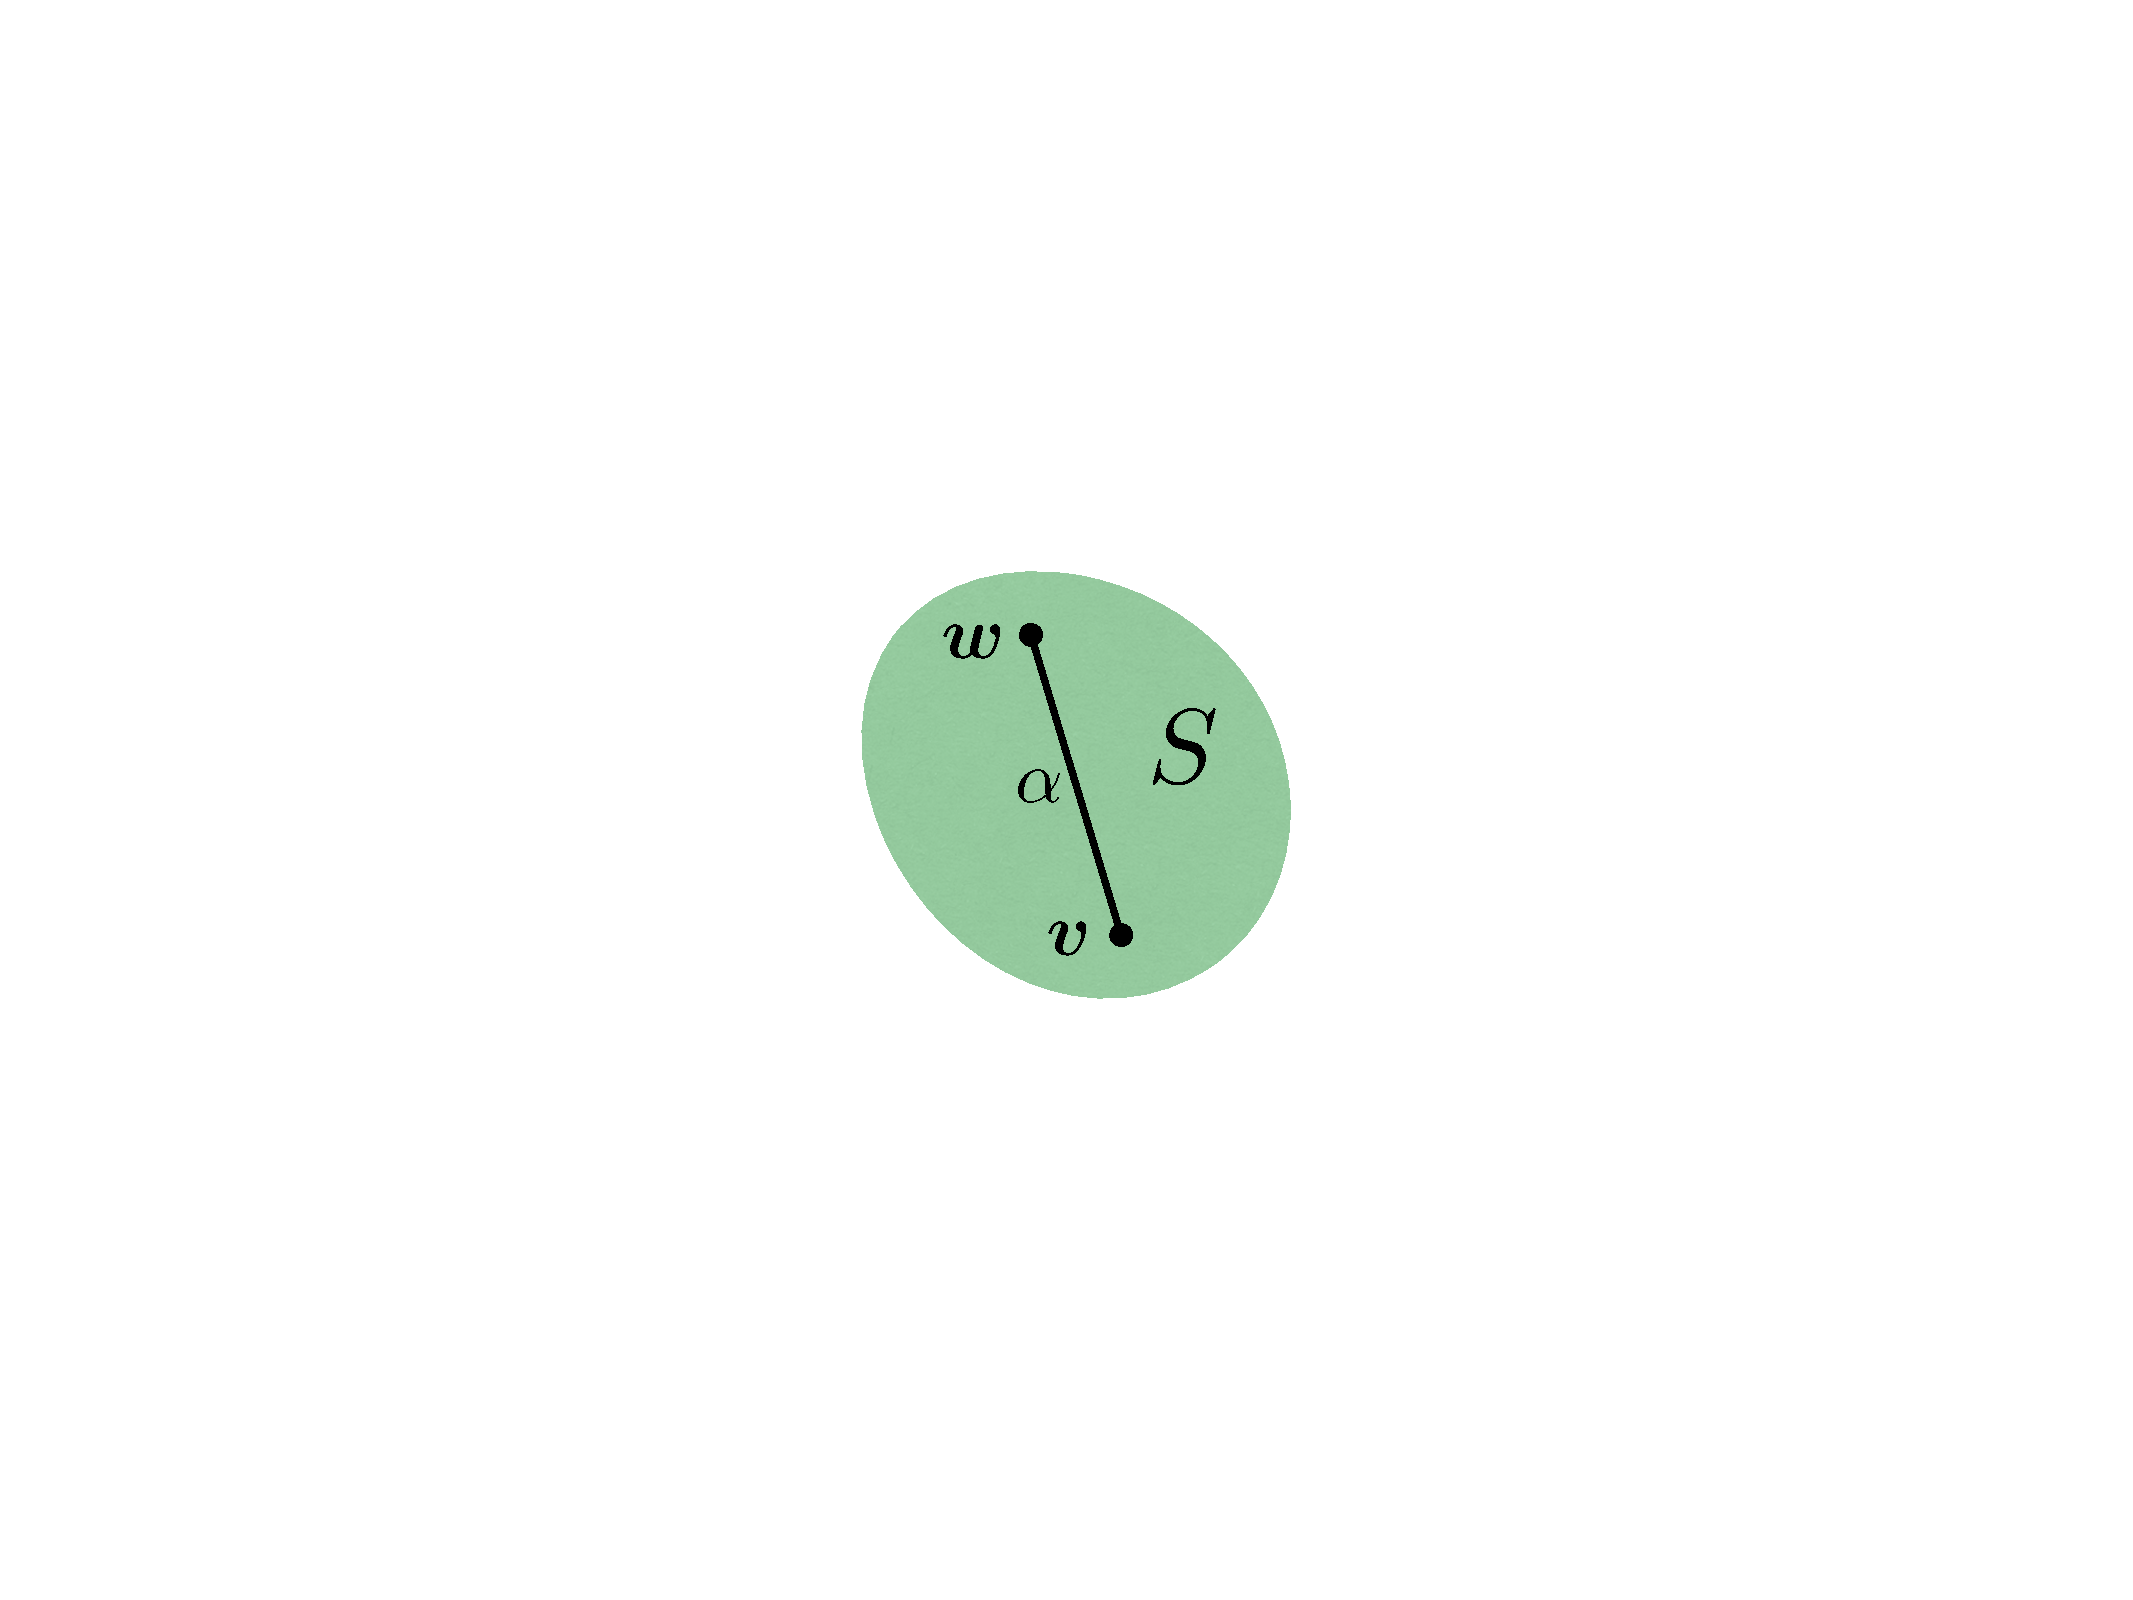
\includegraphics[width=.60\linewidth]{figure/convex_geo.pdf}
    \caption{Convex set visualization}
    \label{fig:convex_geo}
\end{minipage}%
\begin{minipage}{.5\textwidth}
    \centering
    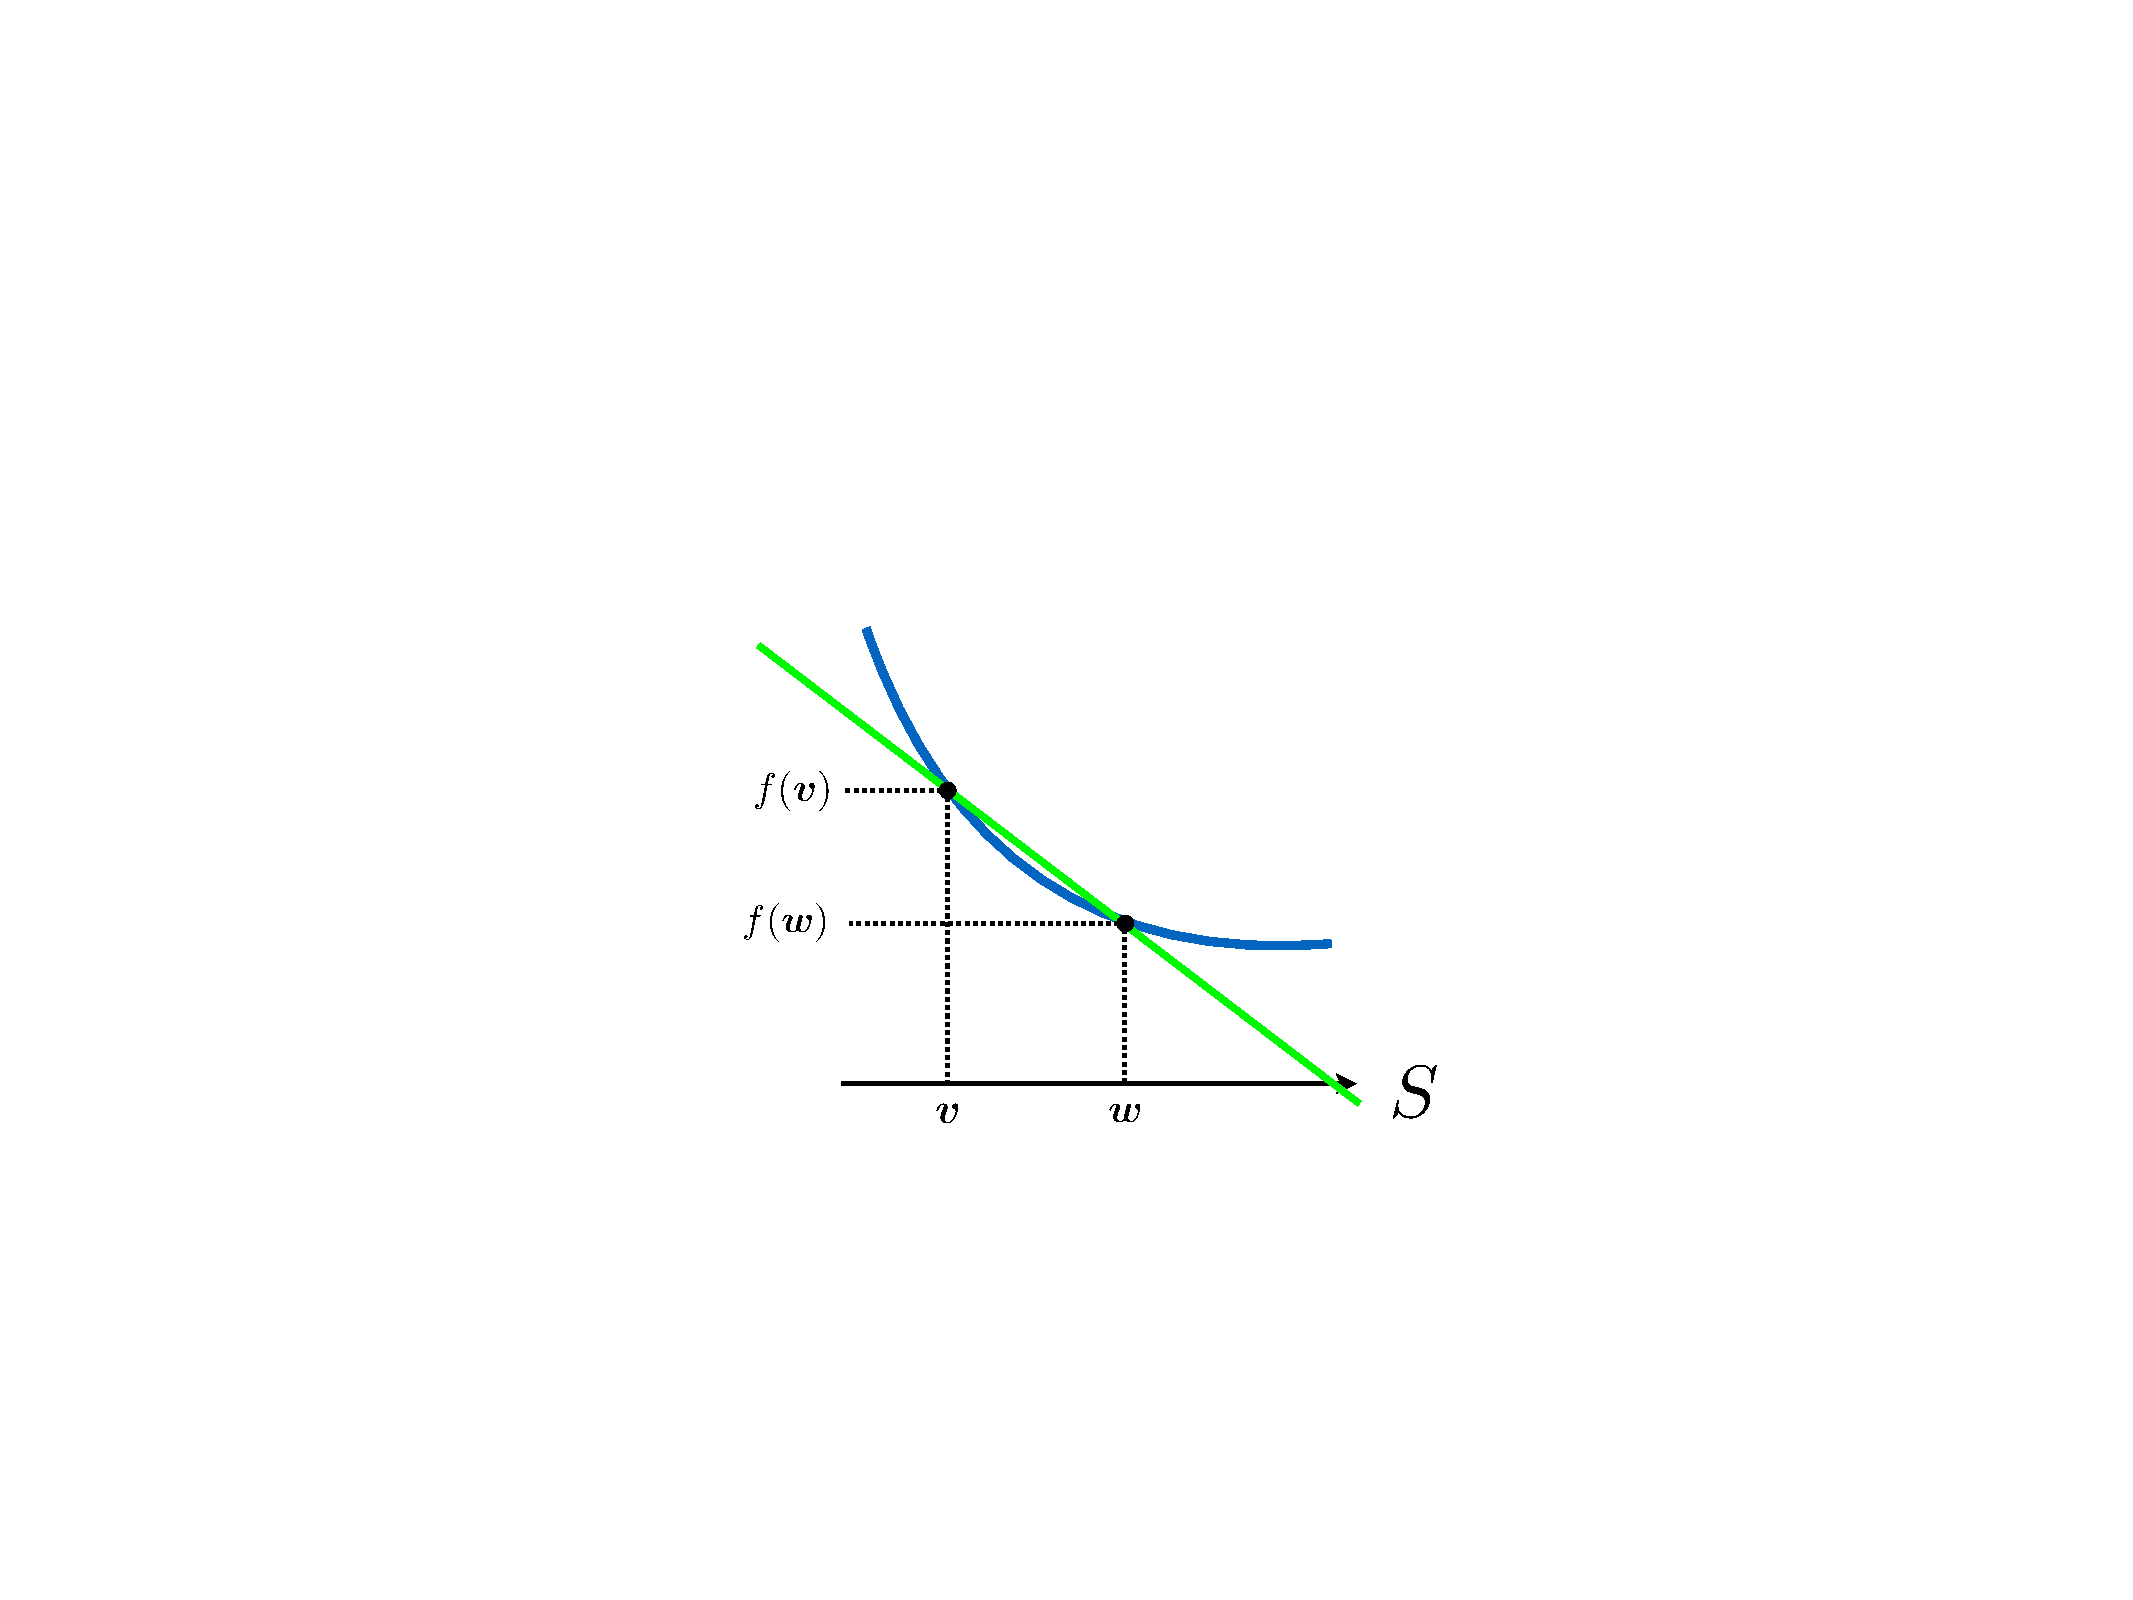
\includegraphics[width=.85\linewidth]{figure/convex_func_geo.pdf}
    \caption{Convex function visualization}
    \label{fig:convex_func_geo}
\end{minipage}
\end{figure}

Convex optimization requires a convex-Lipschitz-bounded (or convex-smooth-bounded) function and a convex solution space. In the next section, we discuss what is \textit{Lipschitz Continuity}.

\subsubsection{Lipschitz Continuity}
A function $f(\cdot)$ is called L-Lipschitz smooth over a set $\mathcal{S}$ with respect to a norm $|| \cdot ||$ if for all $\bm{u}, \bm{w} \in \mathcal{S}$, we have:
\begin{equation}
    \label{eq:lipschitz}
    |f(u) - f(w)| \leq L || \bm{u} - \bm{w} ||
\end{equation}
The inequality (\ref{eq:lipschitz}) describes that the rate of change of function $f$ has to be upper bounded by $L || \bm{u} - \bm{w} ||$ where $L$ is a Lipschitz constant, which limits how fast the function can change. Fig. \ref{fig:lipschitz} shows a good visualization \cite{wiki:lipschitz} of this upper bound: for a Lipschitz-continuous function there exists a double cone (white) that could be moved along the curve without ever intersecting with the curve itself.

\begin{figure}[h]
\centering
\begin{minipage}{.33\textwidth}
    \centering
    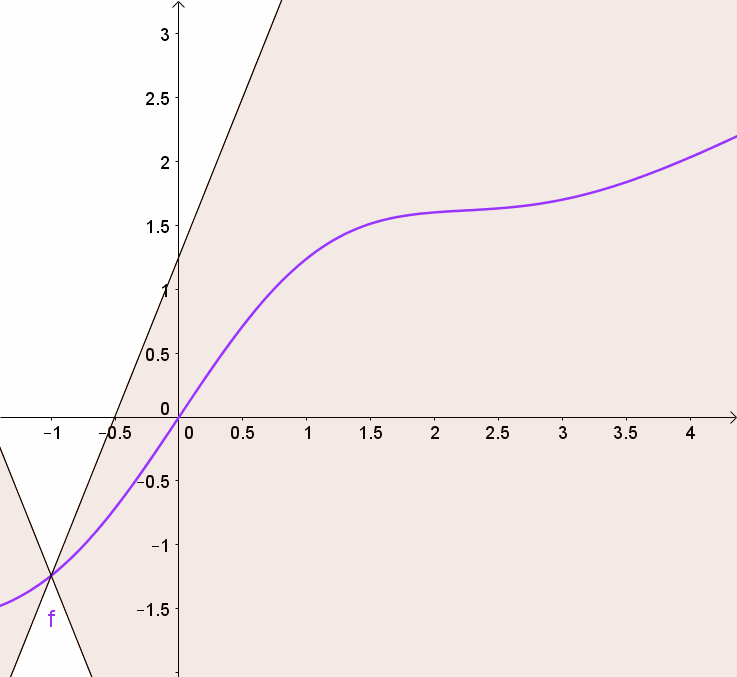
\includegraphics[width=.9\linewidth]{figure/lip_1.png}
\end{minipage}%
\begin{minipage}{.33\textwidth}
    \centering
    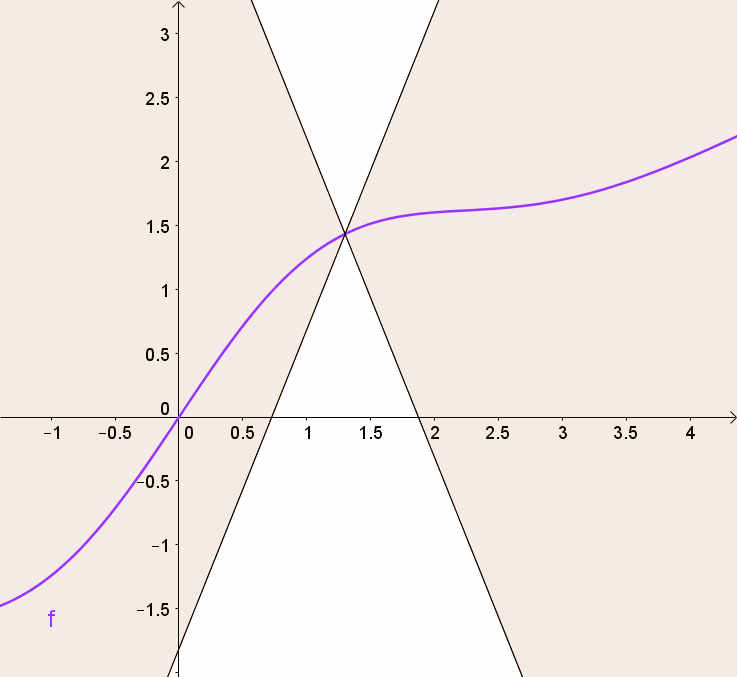
\includegraphics[width=.9\linewidth]{figure/lip_2.png}
\end{minipage}
\begin{minipage}{.33\textwidth}
    \centering
    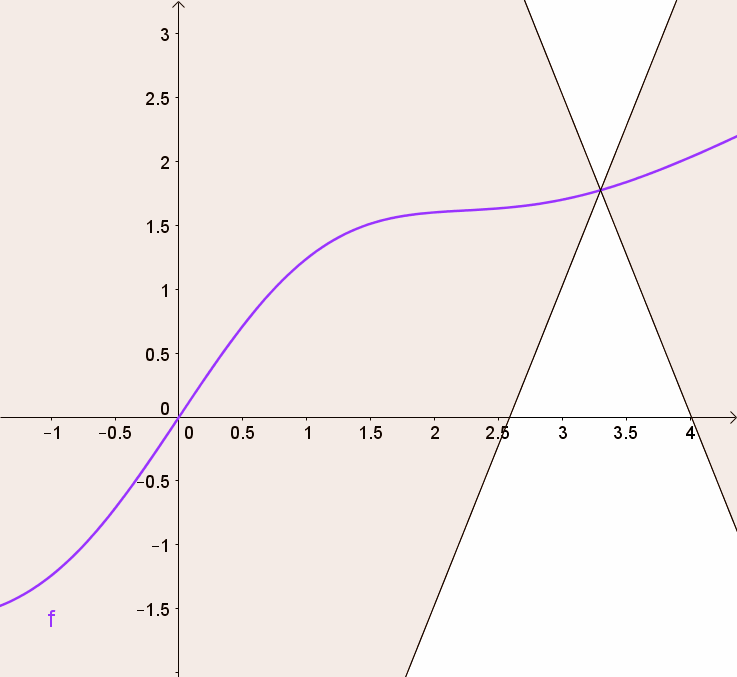
\includegraphics[width=.9\linewidth]{figure/lip_3.png}
\end{minipage}
\caption{Lipschitz continuity visualization \cite{wiki:lipschitz}}
\label{fig:lipschitz}
\end{figure}

Note that the Lipschitz continuity has more to do with the analysis of performance guarantee of the algorithm than whether the optimization will work or not. The Lipschitz constant is a mathematical tool for algorithmic analysis instead of a hyperparameter.

\subsubsection{Convexification}
A loss function is easier to solve when it is convex. If a loss function is not convex, we can use some convexification tricks to make it so. In this section we discuss two methods to convert non-convex loss functions to convex ones.

\begin{addmargin}[2em]{2em}

\textbf{a. Convexification by randomization}\\
Recall the weighted majority algorithm we studied before where we make prediction by taking the sign of inner product between observation and weights:
\begin{equation*}
    \hat{y}^{(t)} = \sign \left \langle \bm{x}^{(t)}, \bm{w}^{(t-1)} \right \rangle
    \label{eq:wma_pred}
\end{equation*}
We define the loss function as:
\begin{equation*}
    l^{(t)} = \mathbf{1}[\hat{y}^{(t)} \neq y^{(t)}]
\end{equation*}
This zero-one loss function is non-convex. Fig. \ref{fig:zero_one_loss}, shows this with an example pair of points forming a segment that passes beneath the function.

\begin{figure}[h]
    \centering
    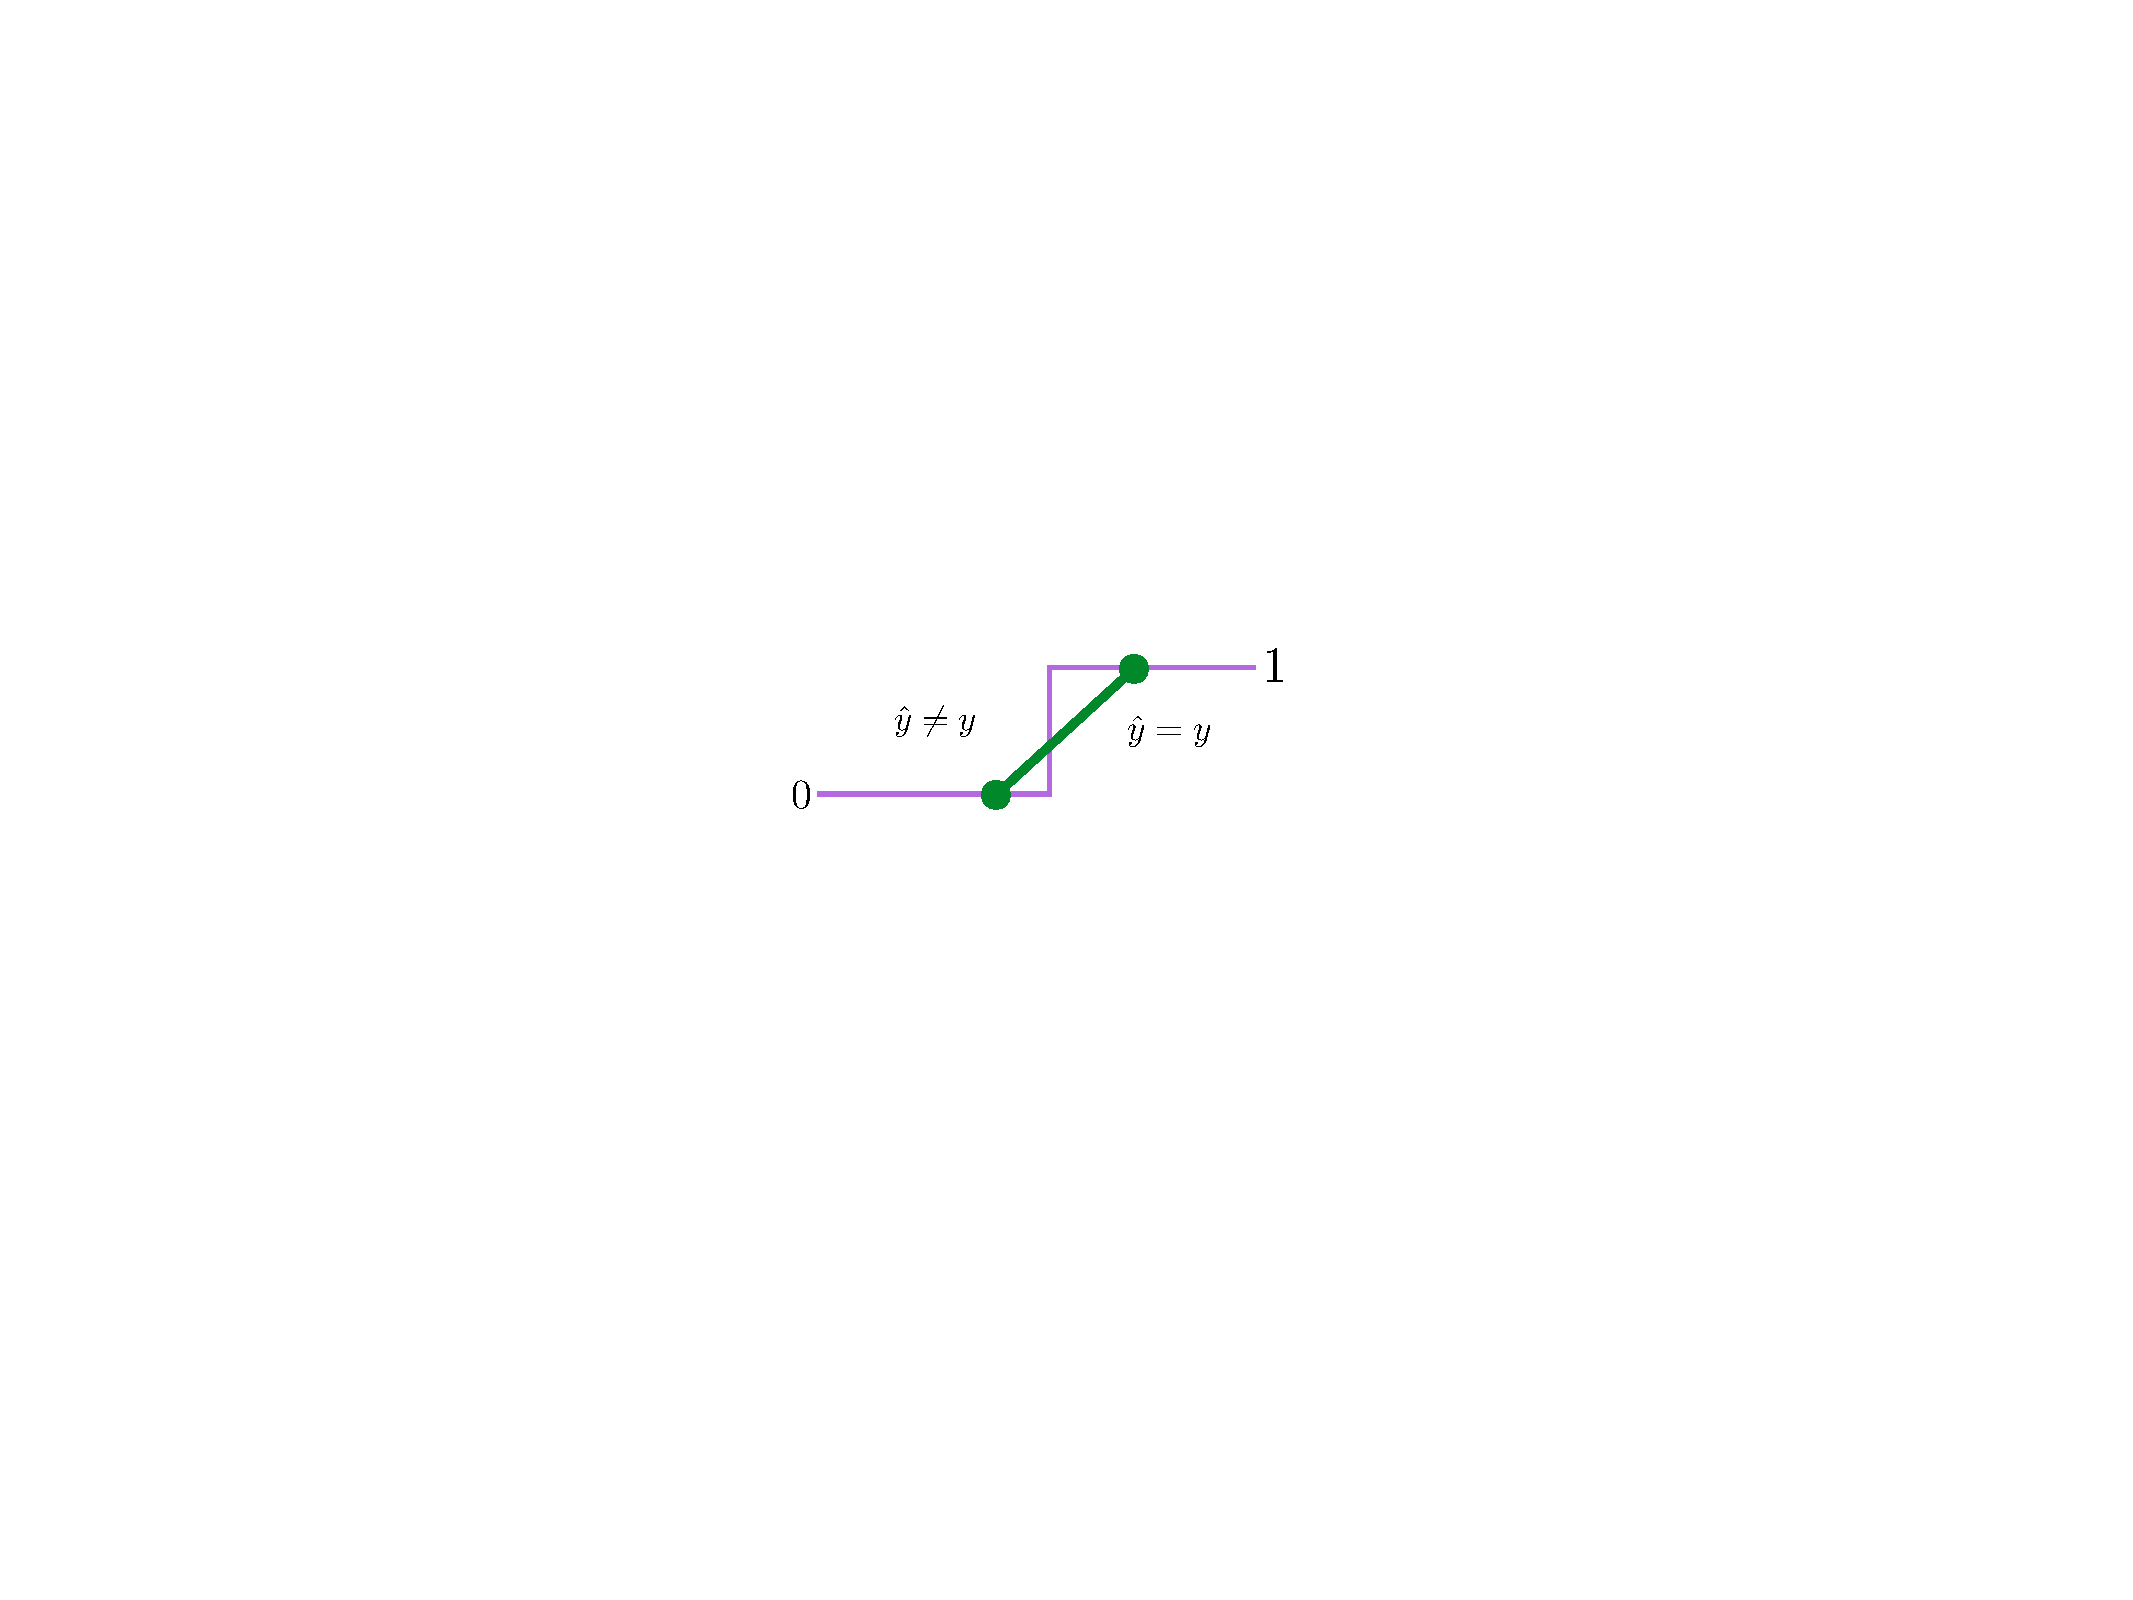
\includegraphics[width=0.4\textwidth]{figure/zero_one_loss.pdf}
    \caption{Zero-one loss function is non-convex}
    \label{fig:zero_one_loss}
\end{figure}

Recall that in randomized weighed majority algorithm, we changed the prediction rule to randomly sample an expert's advice from a multinomial distribution.
% To make the zero-one loss convex, we introduce randomization. Recall that in weighted majority algorithm, we changed the prediction rule by randomly sampling an expert using a multinomial distribution.
\begin{equation*}
    i \sim \textsc{Multinomial} (\bm{w}^{(t-1)} / \bm{\phi}^{(t-1)})
\end{equation*}

It turns out that based on such random sampling, the loss function is changed to be an expectation over the zero-one loss.
\begin{equation*}
    l^{(t)} = E_{\bm{p}}\left[ \mathbf{1}[y^{(t)} \neq \hat{y}^{(t)}] \right] = \sum_{p_n} p_n \cdot \mathbf{1}[y^{(t)} \neq \hat{y}_n^{(t)}]
\end{equation*}
Now because of the expectation, the loss function becomes linear and could take any values between zero and one. Therefore, by doing randomization, we converted the non-convex zero-one loss function to a convex function.

\begin{figure}[h]
    \centering
    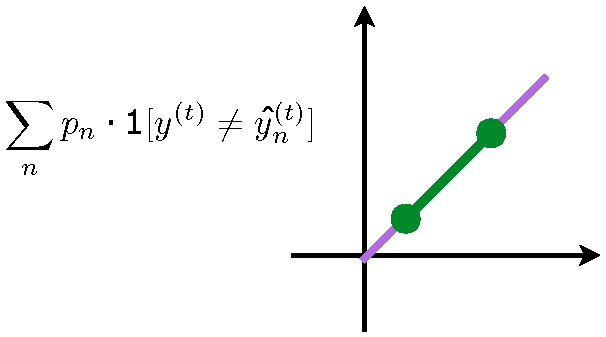
\includegraphics[width=0.4\textwidth]{figure/rwma.pdf}
    \caption{Expectation over zero-one loss function is now convex}
    \label{fig:rwma}
\end{figure}

\textbf{b. Convexification by surrogate loss}\\
Instead of dealing with non-convex loss functions, we can design a convex function that upper-bounds the original loss function and solve the optimization problem using convex optimization infrastructure. This idea is called convexification by surrogate loss. We use the weighed majority algorithm again as an example. The original non-convex zero-one loss function is:
\begin{equation*}
    l^{(t)} = \mathbf{1}[\hat{y}^{(t)} \neq y^{(t)}]
\end{equation*}
We can design a surrogate loss function that upper bounds this loss function to approximate its behavior while making the problem convex. To do so, we need to find a theoretical upper bound for this zero-one loss:
\begin{align*}
    l^{(t)} &= \mathbf{1}[\hat{y}^{(t)} \neq y^{(t)}]\\
            &= \mathbf{1}[-y^{(t)}\hat{y}^{(t)} > 0] && y\text{ is either -1 or 1}\\
            &= \mathbf{1}[-y^{(t)} \langle \bm{w}^{(t-1)}, \bm{x}^{(t)} \rangle > 0] && \text{substitute (\ref{eq:wma_pred})}\\
            &= \mathbf{1}[1-y^{(t)} \langle \bm{w}^{(t-1)}, \bm{x}^{(t)} \rangle > 1] && \text{shift to the right by 1}
    \intertext{
        We can upper bound the original loss function by using a hinge function, as visualized in Fig. \ref{fig:surrogate_loss_hinge}:
    }
    l^{(t)} &= \mathbf{1}[1-y^{(t)} \langle \bm{w}^{(t-1)}, \bm{x}^{(t)} \rangle > 1]\\
            &\leq \max \left[ 0, 1-y^{(t)} \langle \bm{w}^{(t-1)}, \bm{x}^{(t)} \rangle \right] && \text{a convex hinge function } \Tilde{l}^{(t)}
\end{align*}

\begin{figure}[h]
    \centering
    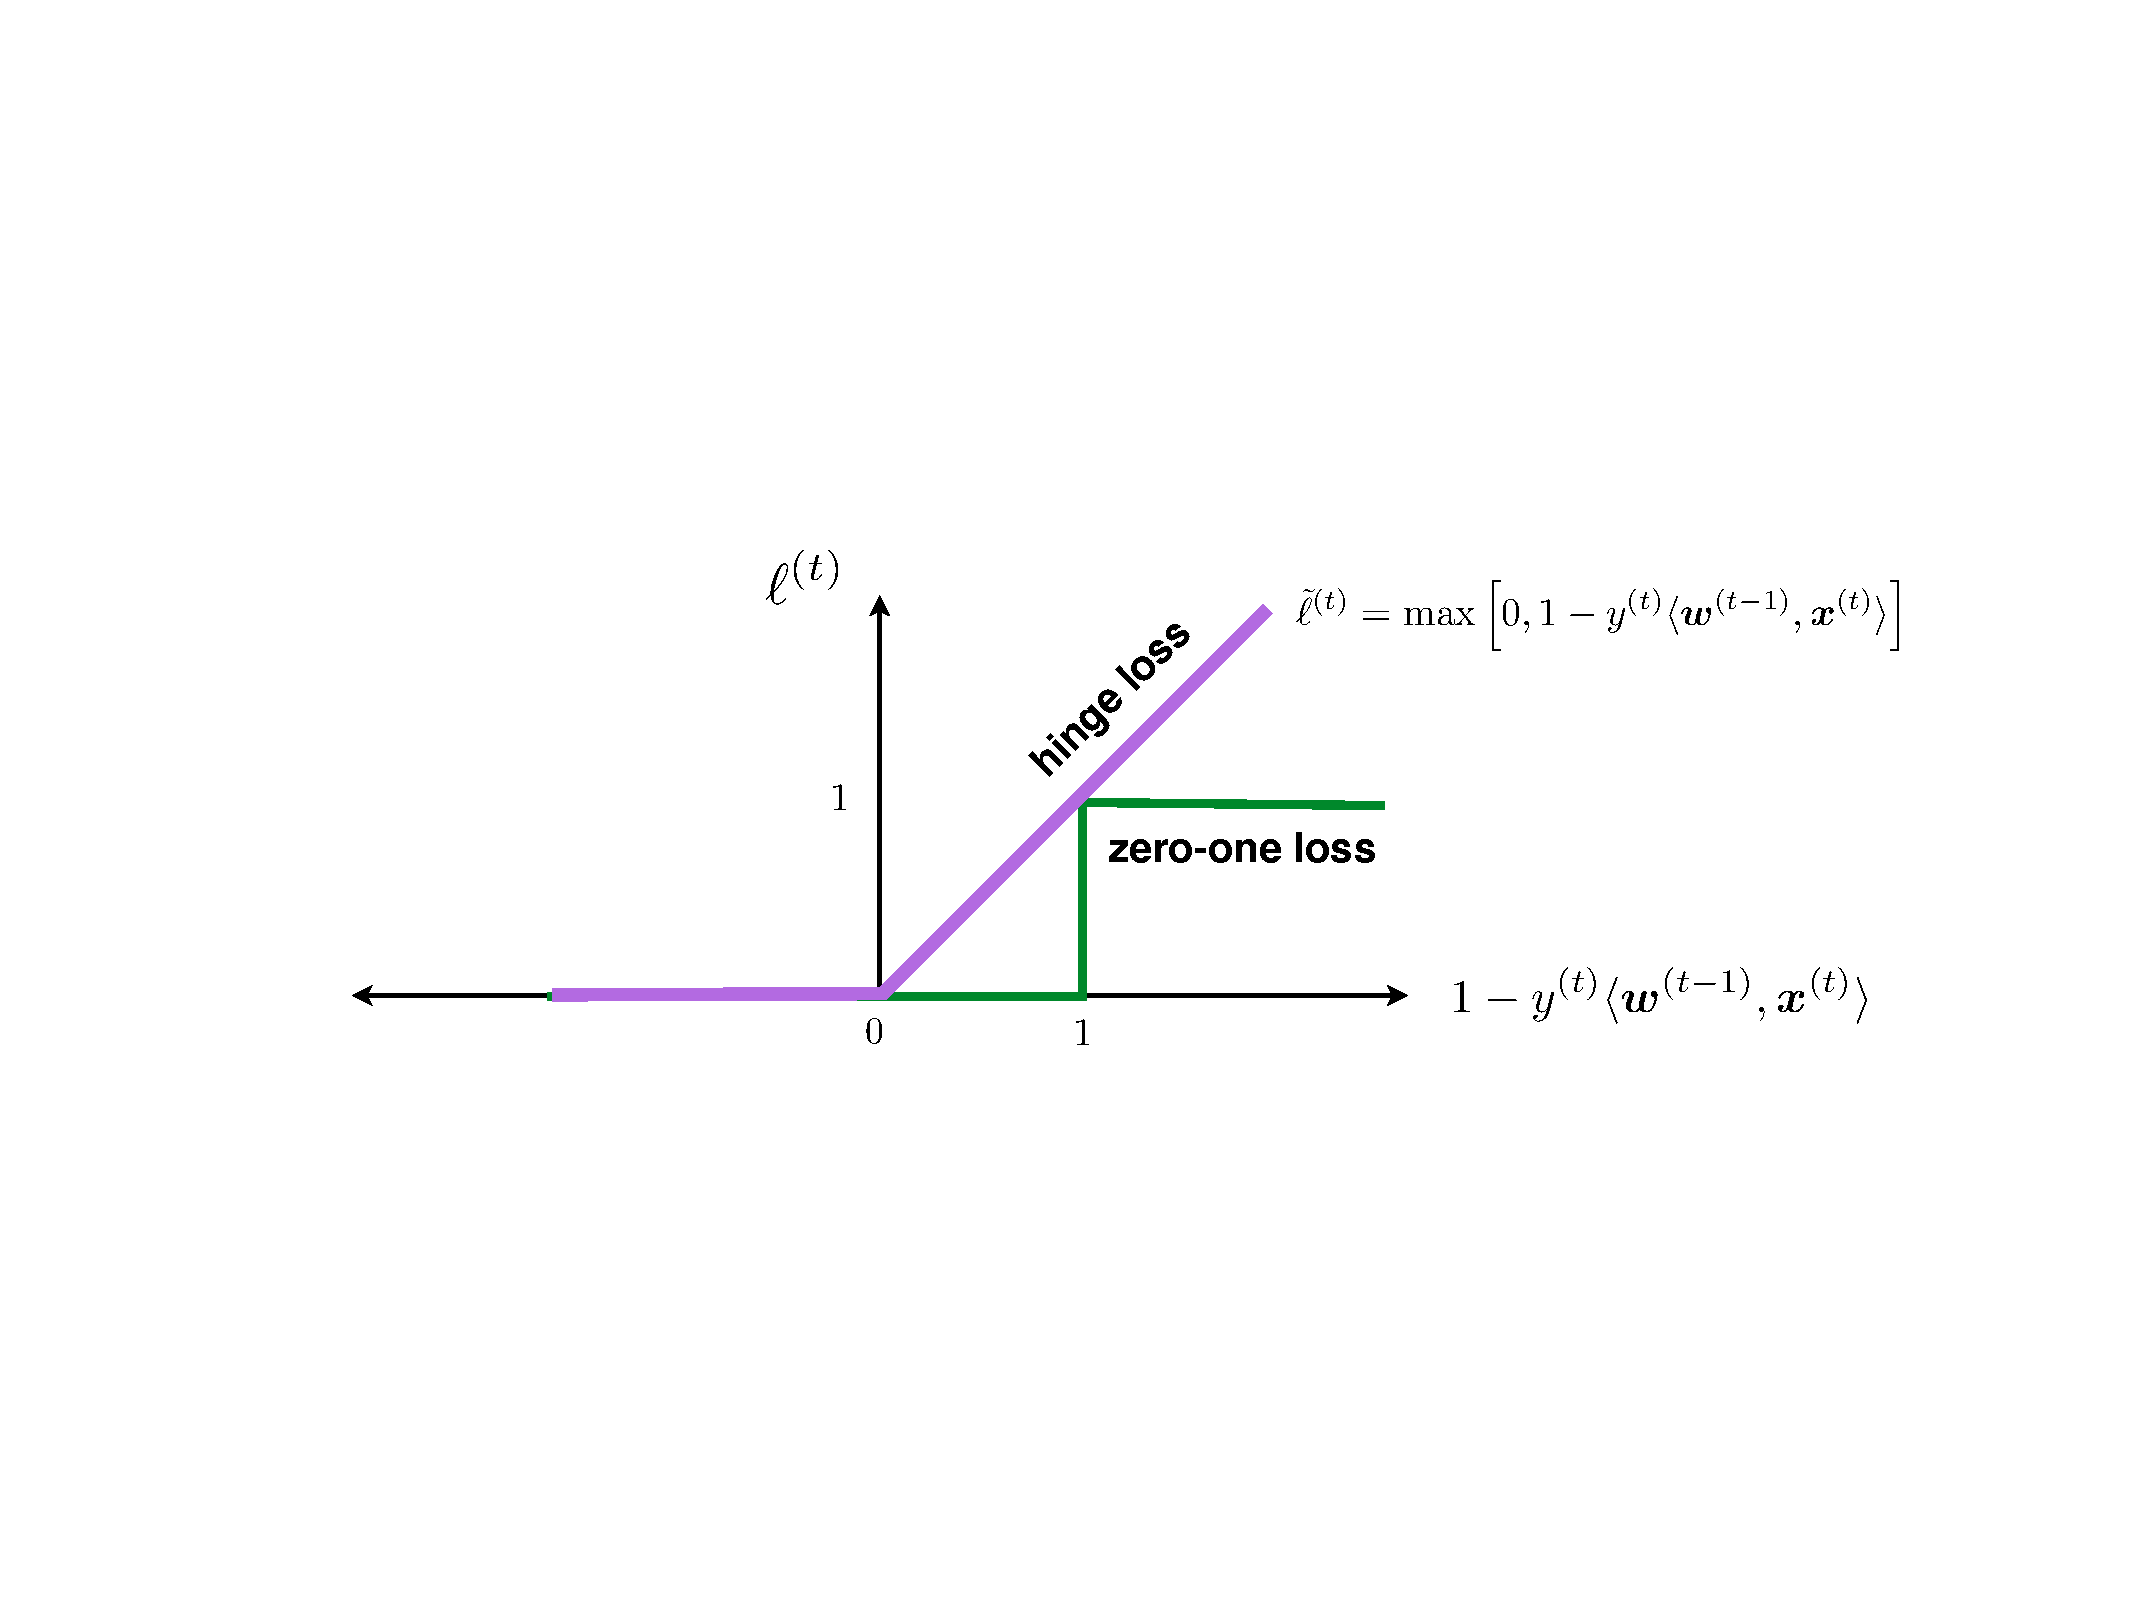
\includegraphics[width=0.9\textwidth]{figure/surrogate_loss_hinge.pdf}
    \caption{The hinge function acts as a surrogate loss for the zero-one loss function by upper-bounding it}
    \label{fig:surrogate_loss_hinge}
\end{figure}

By optimizing the hinge loss $\Tilde{l}^{(t)}$, we have a slightly different behavior than the original zero-one loss especially in the [0, 1] domain where the hinge loss produces non-zero penalty while the original loss function does not. This is a trade-off where we make the optimization easier to solve (using an OCO solver) at the cost of an approximation.

\end{addmargin}

\section{Follow the Leader}
After reviewing the theory part of OCO, we introduce an algorithm called \textit{Follow the Leader} (FTL) known as `Fictitious Play' (Brown 1951 \cite{berger2007brown}). The idea is that the learner select the best choice of the game so far. The FTL pseudocode is listed below.

% \begin{algorithm}[H]
% \caption{Follow The Leader (FTL)}
% \label{algo:ftl}
% \begin{algorithmic}[1]
% \STATE \textbf{function} Follow The Leader
% \FOR{$t=1, 2,\;\cdots,\;T$}
% \STATE $\bm{w}^{(t)}$ = $\argmin{\bm{w} \in W} \Sigma^{t-1}_{i=1} f^{(i)} (\bm{w})$
% \STATE \textsc{Receive} ($f^{(t)} : W \rightarrow \mathbb{R}$)
% \ENDFOR
% \end{algorithmic}
% \end{algorithm}

% \begin{algorithm}
%     \caption{Follow The Leader (FTL)}
%     \label{algo:ftl}
%     \begin{algorithmic}[1]
%     \Function{Follow the Leader}{}
%         \For{\texttt{<some condition>}}
%             \State \texttt{<do stuff>}
%         \EndFor
%     \EndFunction
%   \end{algorithmic}
% \end{algorithm}

\begin{algorithm}
  \caption{Follow the leader algorithm}\label{euclid}
  \begin{algorithmic}[1]
    \Function{Follow the leader}{} %\Comment{The g.c.d. of a and b}
        \For{$t=1, 2,\,\cdots,\;T$}
            \State $\bm{w}^{(t)}$ = $\argmin{\bm{w} \in W} \Sigma^{t-1}_{i=1} f^{(i)} (\bm{w})$ \Comment{Parameter chosen}
            \State \textsc{Receive} ($f^{(t)} : W \rightarrow \mathbb{R}$) \Comment{Receive loss function}
        \EndFor
    \EndFunction
  \end{algorithmic}
\end{algorithm}


The prediction rule is that the learner is going to choose the parameter $\bm{w}$ such that it minimizes the cumulative loss up to now. This rule can be inserted into the online convex optimizer as mentioned in Fig. \ref{fig:oco_1}.

Now we derive a general regret bound for the FTL algorithm. First, we use one-step look ahead cheater to get the regret upper bound. Then we apply algebraic tricks to get the final form.

Recall the definition of cumulative regret:
\begin{equation}
    R(\bm{u}) = \sum_{t}[f^{(t)}(\bm{w}^{(t)}) - f^{(t)}(\bm{u})]
\end{equation}

where $\bm{u}$ is any hypothesis or parameter. Therefore, the cumulative regret is the sum of all the differences between the loss of your online convex optimizer and the loss of hypothesis $\bm{u}$.  

Because hypothesis $\bm{u}$ has infinite possibilities, it is very hard to reason about $\bm{u}$. Therefore, we introduce ``the one-step look ahead cheater'' to upper bound the regret so that we can analyze.   

\begin{equation}
    R(\bm{u}) = \sum_{t}[f^{(t)}(\bm{w}^{(t)}) - f^{(t)}(\bm{u})] \leq \sum_{t}[f^{(t)}(\bm{w}^{(t)}) - f^{(t)}(\bm{w}^{(t+1)})]
\end{equation}

where $\bm{w}^{(t+1)}$ is called ``one-step look ahead cheater''. It means that the prediction rule at step $t$ that has access to parameters of the next iteration $t+1$. We don't have access to the parameters of the future. However, we can use theoretical values to enable the analysis. The ``one-step look ahead cheater'' gives us the access to future observations/loss that enables the computation of the best $\bm{w}$. 

To prove the inequality (3), by subtracting $f^{(t)}(\bm{w}^{(t)})$ from both sides, we only need to prove that:
\begin{equation}
    \sum_{t=1}^{T} f^{(t)}(\bm{w}^{(t+1)}) \leq \sum_{t=1}^{T}f^{(t)}(\bm{u})
\end{equation}

If it holds true, it means that the loss of a series of one step cheaters is not larger than the loss of any other single parameter $\bm{u}$. Therefore, our claim is:
\begin{equation}
    \sum_{t=1}^{T} f^{(t)}(\bm{w}^{(t+1)}) \leq \sum_{t=1}^{T}f^{(t)}(\bm{u}) \quad \forall \bm{u}
\end{equation}

Proof. By induction method, we first assume our claim is true for $T-1$ and will prove it holds true for $T$:
\begin{equation}
    \sum_{t=1}^{T-1} f^{(t)}(\bm{w}^{(t+1)}) \leq \sum_{t=1}^{T-1}f^{(t)}(\bm{u})
\end{equation}

Then we add $f^{(T)}(\bm{w}^{(T+1)})$ to both sides of inequality (6), where $f^{(T)}(\bm{w}^{(T+1)})$ is the loss of the one step look ahead cheater for the next time step, we can get:
\begin{equation}
    \sum_{t=1}^{T} f^{(t)}(\bm{w}^{(t+1)}) \leq \sum_{t=1}^{T-1}f^{(t)}(\bm{u}) + f^{(T)}(\bm{w}^{(T+1)})
\end{equation}

Since the inequality (7) holds true for all $\bm{u}$, if we let $\bm{u} = \bm{w}^{(T+1)}$, we can get:
\begin{equation}
    \sum_{t=1}^{T} f^{(t)}(\bm{w}^{(t+1)}) \leq \sum_{t=1}^{T-1}f^{(t)}(\bm{w}^{(T+1)}) + f^{(T)}(\bm{w}^{(T+1)})
\end{equation}
\begin{equation}
    \sum_{t=1}^{T} f^{(t)}(\bm{w}^{(t+1)}) \leq \sum_{t=1}^{T}f^{(t)}(\bm{w}^{(T+1)})
\end{equation}

It means that the loss of always using one step look ahead cheater is the lower bound of the loss of using a single cheater at the end of the
sequence for all time steps. Recall the minimizer by definition,
\begin{equation}
    \bm{w}^{(T+1)} = \argmin{\bm{u} \in S} \sum^{T}_{t=1} f^{(t)}(\bm{u})
\end{equation}

This means the right hand side of the inequality (9) can be upper bounded by $\sum^{T}_{t=1} f^{(t)}(\bm{u})$. Therefore, we have
\begin{equation}
    \sum_{t=1}^{T} f^{(t)}(\bm{w}^{(t+1)}) \leq \sum^{T}_{t=1} f^{(t)}(\bm{u})
\end{equation}
Therefore, it proves our claim and the inequality (3). 

% \begin{algorithm}[H]
% \SetAlgoLined
% \DontPrintSemicolon
% \KwIn{$ F $\Comment*[r]{List of Sensitive Terms}}    
% \KwOut{$ S^{*} $ \Comment*[r]{Negation Excluded List}}

%     \SetKwFunction{FMain}{NegationDetection}
%     \SetKwProg{Fn}{Function}{:}{}
%     \Fn{\FMain{$F$}}{
%         $ S^{*}  \longleftarrow F $;    

%         \ForEach{$ F \in NPs $}
%         {\eIf{$ f_i = Negated $}
%             {$ N \longleftarrow f_i;$}
%             {$ S \longleftarrow f_i;$}

%         }
%         \textbf{return} $ S^{*}; $ 
% }
% \textbf{End Function}
% \caption{Algorithm for Excluding the Negation}
% \label{NagetionAlgo}
% \end{algorithm}



%\section*{References}
%Include your references here. Please cite any resources you found useful.	
%Populate the refs.bib file or list your references manually. Be consistent in formatting!
{
\bibliography{refs}
\bibliographystyle{abbrv}
}

%\section{Appendix}
%This section provides any relevant background material that was not covered in the lectures, but was found to be useful for understanding the material. 
%For example, derivations, theory underlying techniques employed, etc. 

%Additionally, this section can summarizes applications or extensions of these techniques found in the literature. 

\end{document} % Done!





